%%
%% This is file `thesis-ex.tex',
%% generated with the docstrip utility.
%%
%% The original source files were:
%%
%% uiucthesis2009.dtx  (with options: `example')
%% 
\def\fileversion{v2.25a} \def\filedate{2013/04/17}
%% Package and Class "uiucthesis2009" for use with LaTeX2e.
\documentclass[edeposit,10pt,fullpage]{uiucthesis2009}

\usepackage{amsmath, amsthm, amssymb}
\usepackage[numbers]{natbib}

\usepackage{color}
\usepackage{verbatim}

\usepackage{subfigure}
\usepackage{url}
\usepackage{times}
\usepackage{mathptmx}
\usepackage[ruled,vlined]{algorithm2e}
\usepackage[pdftex]{graphicx}
\usepackage{booktabs}

\usepackage{subfigure}
\usepackage{caption}
\usepackage{longtable}
\usepackage{tikz}
\usetikzlibrary{arrows,positioning,fit,scopes}
\usetikzlibrary{shapes.multipart}

\colorlet{d}{black!25}
\colorlet{l}{black!0}
\newcommand{\btnode}[4]{ \nodepart{#1} #2\\ $[$#3,#4) }
\newcommand{\btplainnode}[2]{ \nodepart{#1} #2  \\  }
\tikzset{nd/.style={rectangle split, rectangle split parts=3, draw=black!75, thick,
            rectangle split horizontal, align=center, rectangle split empty part width=0.5cm,
            rectangle split part fill={#1}}}

\usepackage[pdfborder={0 0 0}]{hyperref}

\interfootnotelinepenalty=10000  % Split footnote are annoying

\newcommand{\ntaskip}{\vspace{-0.15in}}
\SetAlgoSkip{ntaskip}

\newenvironment{captiontext}{%
   \begin{center}%
     \begin{minipage}{0.99\linewidth}%
       \renewcommand{\baselinestretch}{0.9}%
         \sffamily\footnotesize}%
   {\renewcommand{\baselinestretch}{1.0}%
      \end{minipage}%
        \end{center}}

\newenvironment{smitemize}%
  {\begin{list}{$\bullet$}%
     {\setlength{\parsep}{0pt}%
      \setlength{\topsep}{0pt}%
      \setlength{\itemsep}{2pt}}}%
  {\end{list}}

\clubpenalty=10000  % Don't allow orphans
\widowpenalty=10000 % Don't allow widows

% \raggedbottom

\renewcommand{\textfraction}{0}
\renewcommand{\topfraction}{1}
\renewcommand{\bottomfraction}{1}
\setcounter{totalnumber}{10}
\setcounter{topnumber}{10}
\setcounter{bottomnumber}{10}
\setcounter{dbltopnumber}{10}
\renewcommand{\floatpagefraction}{1}
\renewcommand{\dblfloatpagefraction}{1}

%Remove this at the end.
\newcommand{\citetemp}[1]{(#1)}
\newcommand{\temp}[1]{?#1?}

\begin{document}

\title{Android Behind the Scenes. Revealing Hidden Malware with AndroMEDA}
\author{Robert Joseph Marsan}
\department{Computer Science}
\schools{M.S, University of Illinois at Urbana-Champaign, 2013}
\msthesis
\advisor{Roy H. Campbell}
\degreeyear{2013}
\committee{Professor Roy H. Campbell}
\maketitle

\frontmatter

%% Create an abstract that can also be used for the ProQuest abstract.
%% Note that ProQuest truncates their abstracts at 350 words.
\begin{abstract}
The tremendous rise of mobile computing has led to an equally strong rise in mobile malware. Android, the predominant mobile OS, uses a Permission based security system that is ill equipt to deal with many forms of malware, especially Info Theft Malware. To better understand the issue, we introduce the concept of the User-App Agreement - a framework for a user consenting and trusting specific actions an app may take. Using this concept, we examine the Android Permission system with Android Census - a comprehensive app metadata database - and conclude the main pitfall lies in the Permission system's lack of addressing context and use. Finally, we present AndroMEDA, an Android Security Extension which helps provide an understanding of context and use of Android Permissions to users, allowing them to make better judgment over whether actions are trusted or not. We demonstrate how this can be used to mitigate sophisticated Info Theft Malware.

\end{abstract}

%% Create a dedication in italics with no heading, centered vertically
%% on the page.
\begin{dedication}
To my\\
Parents, Lisa and Mark
\end{dedication}

%% Create an Acknowledgements page, many departments require you to
%% include funding support in this.
\chapter*{Acknowledgments}

I would like to express my most sincere gratitude towards my advisor Roy H. Campbell for his continuous guidance and support of my work, as well as Lynette Lubben for her patience. Roy and Lynette opened many doors for my research, and I could not be more appreciative.

I cannot find the words to express my gratitude towards Alejandro Gutierrez for his tireless support and assistance, and unwavering confidence and dedication. My research would not be what it is today without his contributions and mentorship. %The man's dedication is severely underappreciated, and I hope he sleeps sometime. 

%I need to thank the department but I'm not sure 

%% The thesis format requires the Table of Contents to come
%% before any other major sections, all of these sections after
%% the Table of Contents must be listed therein (i.e., use \chapter,
%% not \chapter*).  Common sections to have between the Table of
%% Contents and the main text are:
%%
%% List of Tables
%% List of Figures
%% List Symbols and/or Abbreviations
%% etc.

\tableofcontents
\listoftables
\listoffigures

%this can add another section...?
%\addcontentsline{toc}{chapter}{List of Algorithms}

%% Create a List of Abbreviations. The left column
%% is 1 inch wide and left-justified
%\chapter{List of Abbreviations}
%
%\begin{symbollist*}
%\item[CA] Caffeine Addict.
%\item[CD] Coffee Drinker.
%\end{symbollist*}

%% Create a List of Symbols. The left column
%% is 0.7 inch wide and centered
%\chapter{List of Symbols}

%\begin{symbollist}[0.7in]
%\item[$\tau$] Time taken to drink one cup of coffee.
%\item[$\mu$g] Micrograms (of caffeine, generally).
%\end{symbollist}

\mainmatter

\chapter{Introduction}
\label{sec:intro}

%\textbf{Thesis Statement}: Malware, and especially Info Theft Malware, on Mobile Operating Systems, especially Android, is better understood when not just analyzing the capabilities of an application, but the expectations the user has as to how it utilizes those capabilities as well.\\
%\textbf{Thesis Statement}: Android Malware detection is complemented by not just analyzing the capabilities of an app, but the context and use as well.\\
%\textbf{Thesis Statement}: In order to detect Android Malware, the user must understand what is going on behind the scenes of the app. The capabilities of an app are important, but the context and use of these capabilities are as well.\\
\textbf{Thesis Statement}: Using a novel feedback loop, we provide users with a method for understanding the context and use of actions an app performs, thus allowing them to identify suspicious behavior that violates users' trust.\\


The rise of smartphones in the last decade years has been unprecedented. Since the launch of the Apple iPhone in 2007, there are now almost 1 Billion smartphone users in the world\citep{kpcbinternetreport2012}. These new devices marked an unprecedented shift in our relationship with computers, becoming the center point for many personal endeavors, and superseding almost all previous computing devices from cell phones, to cameras, to GPS devices, and to most uses of a desktop PC\citep{hua2012introduction}. Smartphones continue to become the focal point of almost all personal computing, and consequently the operating systems they run become more important and powerful.

\section{Contributions}
In this thesis, we highlight 4 key areas:
\begin{smitemize}
\item \textit{User-App Agreement}: First, we discuss the challenges of addressing modern mobile malware, and the shortcomings of the Android security model. We introduce the User-App Agreement (UAA), a way of conceptualizing the trust a user has in actions an applications may perform, as a key component in identifying malicious behavior.
\item \textit{Android Census}: Second, we use a novel dataset, Android Census, to examine the state of Android permissions. We find Android permissions correlate with expected use, but key examples are shown of less than legitimate use. Using a comprehensive set of malware, we cross examine how the permissions of malware compares with the Android Census. We conclude that malware that targets the user's personal information is the most difficult to detect using this static analysis.
\item \textit{IncognitoWare}: Third, we address the shortcomings of the current malware datasets available to academia, and introduce a new dataset of IncognitoWare. This dataset is more representative of current trends in malware, and proves to be a great challenge to detect.
\item \textit{AndroMEDA}: Finally, we introduce Android Malware Evaluation Detection and Analysis (AndroMEDA), a set of Android extensions, and a companion app, build off of the premise of the User-App Agreement. By giving the user more information on the context and use of sensitive system actions, they can evaluate whether they trust those actions, and ultimately whether the app is acting maliciously or not.
\end{smitemize}
\subsection{}





% After untrusted behavior is spotted, the actions can be reported, and knowledge can be spread to all users. All of this makes users more aware of app behavior, and helps mitigate Info Theft Malware on Android.

%Building off the concept of the User-App Agreement, we introduce AndroMEDA. Key parts of the User-App Agreement were previously unnoticable to the user until AndroMEDA. By giving the user more information on the context and use of permissions, they can evaluate whether they trust those actions, and ultimately whether the app is acting maliciously or not. After untrusted behavior is spotted, the actions can be reported, and knowledge can be spread to all users. All of this makes users more aware of app behavior, and helps mitigate Info Theft Malware on Android.


%This security model has dramatically changed the nature of mobile software, and in turn, mobile malware. By forcing malware to fit inside of this security sandbox, malware authors must choose to either break out of the box, or work inside of it. This constriction has blurred the definition of mobile malware, and ultimately has profound implications for the user of the mobile device. We will examine these implications, and propose new tools and methods to help understand the nuances of modern malware, as well as provide a framework of tools to detect them.


\chapter{Background \& Motivation}
\label{sec:background}

%To understand the nature of modern mobile malware, we first examine the context. The two main models, that of iOS and Android, are compared and contrasted here.

\section{The ``App'' and Sandboxing}

In the mobile world, ``Apps'' are isolated and sandboxed programs, generally designed with one singular purpose. They lack dependencies, and generally are not as privileges as system software for performing many tasks. The mechanisms for accessing functionality outside of their sandbox is enforced by a set of policies the system holds, specific to that app. On some platforms, like iOS, only one app may run at any given time, and background computation is virtually non-existent (with some exceptions)\footnote{Minor amounts of computation can be done to compute background audio, and other isolated background tasks.}, along with many other restrictions. On Android and other platforms, many more features are available to apps, but in all cases, the ``app'' lifecycle is well defined and controlled by the system much more than on a PC OS.

There are various reasons for the tight sandboxing of mobile apps. Power and resource consumption are certainly a factor - mobile OSs generally reserve the right to kill apps if they attempt to allocate too much memory. Controlling access to hardware also helps in this: allowing apps to keep the phone awake could easily drain battery. However, another reason for sandboxing, and arguably more important, is protecting Personally Identifiable Information.

\subsection{Personally Identifiable Information}

Personally Identifiable Information (PII), as defined by the National Institute of Standards and Technology, is ``any information about an individual maintained by an agency, including (1) any information that can be used to distinguish or trace an individual‘s identity... and (2) any other information that is linked or linkable to an individual'' \citep{mccallister2010guide}. Mobile devices, having blended cameras, cell phones, GPS devices, and PCs into one device, have an extremely diverse amount of PII, from phone numbers, to contacts, to location history, to bank account numbers and pictures. For many of these datasets, mobile OSs actually organize them into databases with the intention of allowing 3rd parties access to them. Contact lists, SMS, Photographs and location history are available to apps on virtually every mobile platform in some official way. This is a driving motivation for a greatly improved security model for mobile OSs: controlling 3rd party software's access to PII. 

% Expand more on this.

\subsection{Digital Distribution Platform}

The final major difference between mobile OSs and PC OSs is the distribution of code. No mobile OS allows 3rd party code to be ran outside of the sandbox, and all of them require the user's consent before installing an app. All apps must be signed, and in general, there is 1 main distribution channel for all apps on a mobile OS. This tightly controlled distribution both aids in security, as well as controls the ecosystem around that mobile OS.

\subsection{Apple's App Store}
The first major digital distribution platform for mobile apps was Apple's App Store\citep{AppleAppStore}. It's model has been repeated by almost all major mobile app distribution platforms. The basic premise is simple: developers sign up to the app store, pay a fee (usually yearly), and submit fully-finished apps. A reviewer runs the app in a monitored sandbox, watches for unusual behavior, checks for stability and usability, and approves it. Once the app has been approved, it's released onto the app store, at which time anyone can download it. The approval process, as well as the high monetary fee, act as a way to ensure only safe and high-quality apps are available for that platform. In this type of platform, typically no apps may be installed from other sources. On iOS, initially this was the main method of security: if the app passed the inspection, it was acknowledged as safe and virtually unmonitored unless someone noticed something unusual and reported it. However, in recent years, after certain incidents (see section \ref{sec:path}), apps still must request permission from the user to perform certain tasks.

\subsection{Android Permissions}
Android's distribution platform takes a different approach, and at it's core is also Android's security model: The Permission System (see section \ref{sec:permissions}). Android Apps declare when they are packaged what capabilities they will use, and the user reviews them at install time. If the user approves the app, it may use the requested capabilities whenever it wants: little restrictions are placed otherwise. With this barrier in mind, the Google Play Store (formerly known as the Android Market), or GPStore, opts for an alternate model to iOS, where the developer pays a smaller fee, and apps go through no formal approval process. After an app's submission, it's immediately released into the wild for users to download and run. The assumption Android uses is that the metadata the GPStore provides: App name, Developer Name, Description, Reviews and Ratings, are enough for the user to determine if the app should be trusted with the permission set it's given (see Figure \ref{fig:gpstoreapps}). In fact, Android even allows the device to accept apps from 3rd party sources, a practice known as ``sideloading'', although it's disabled by default. This has spawned a large number of 3rd party app sources, all of which rely on the Permission system for user protection.

%GPSTORE IMAGE AND CHART EXPLAINING THE LETTERS.

\begin{figure}[h]
\begin{center}
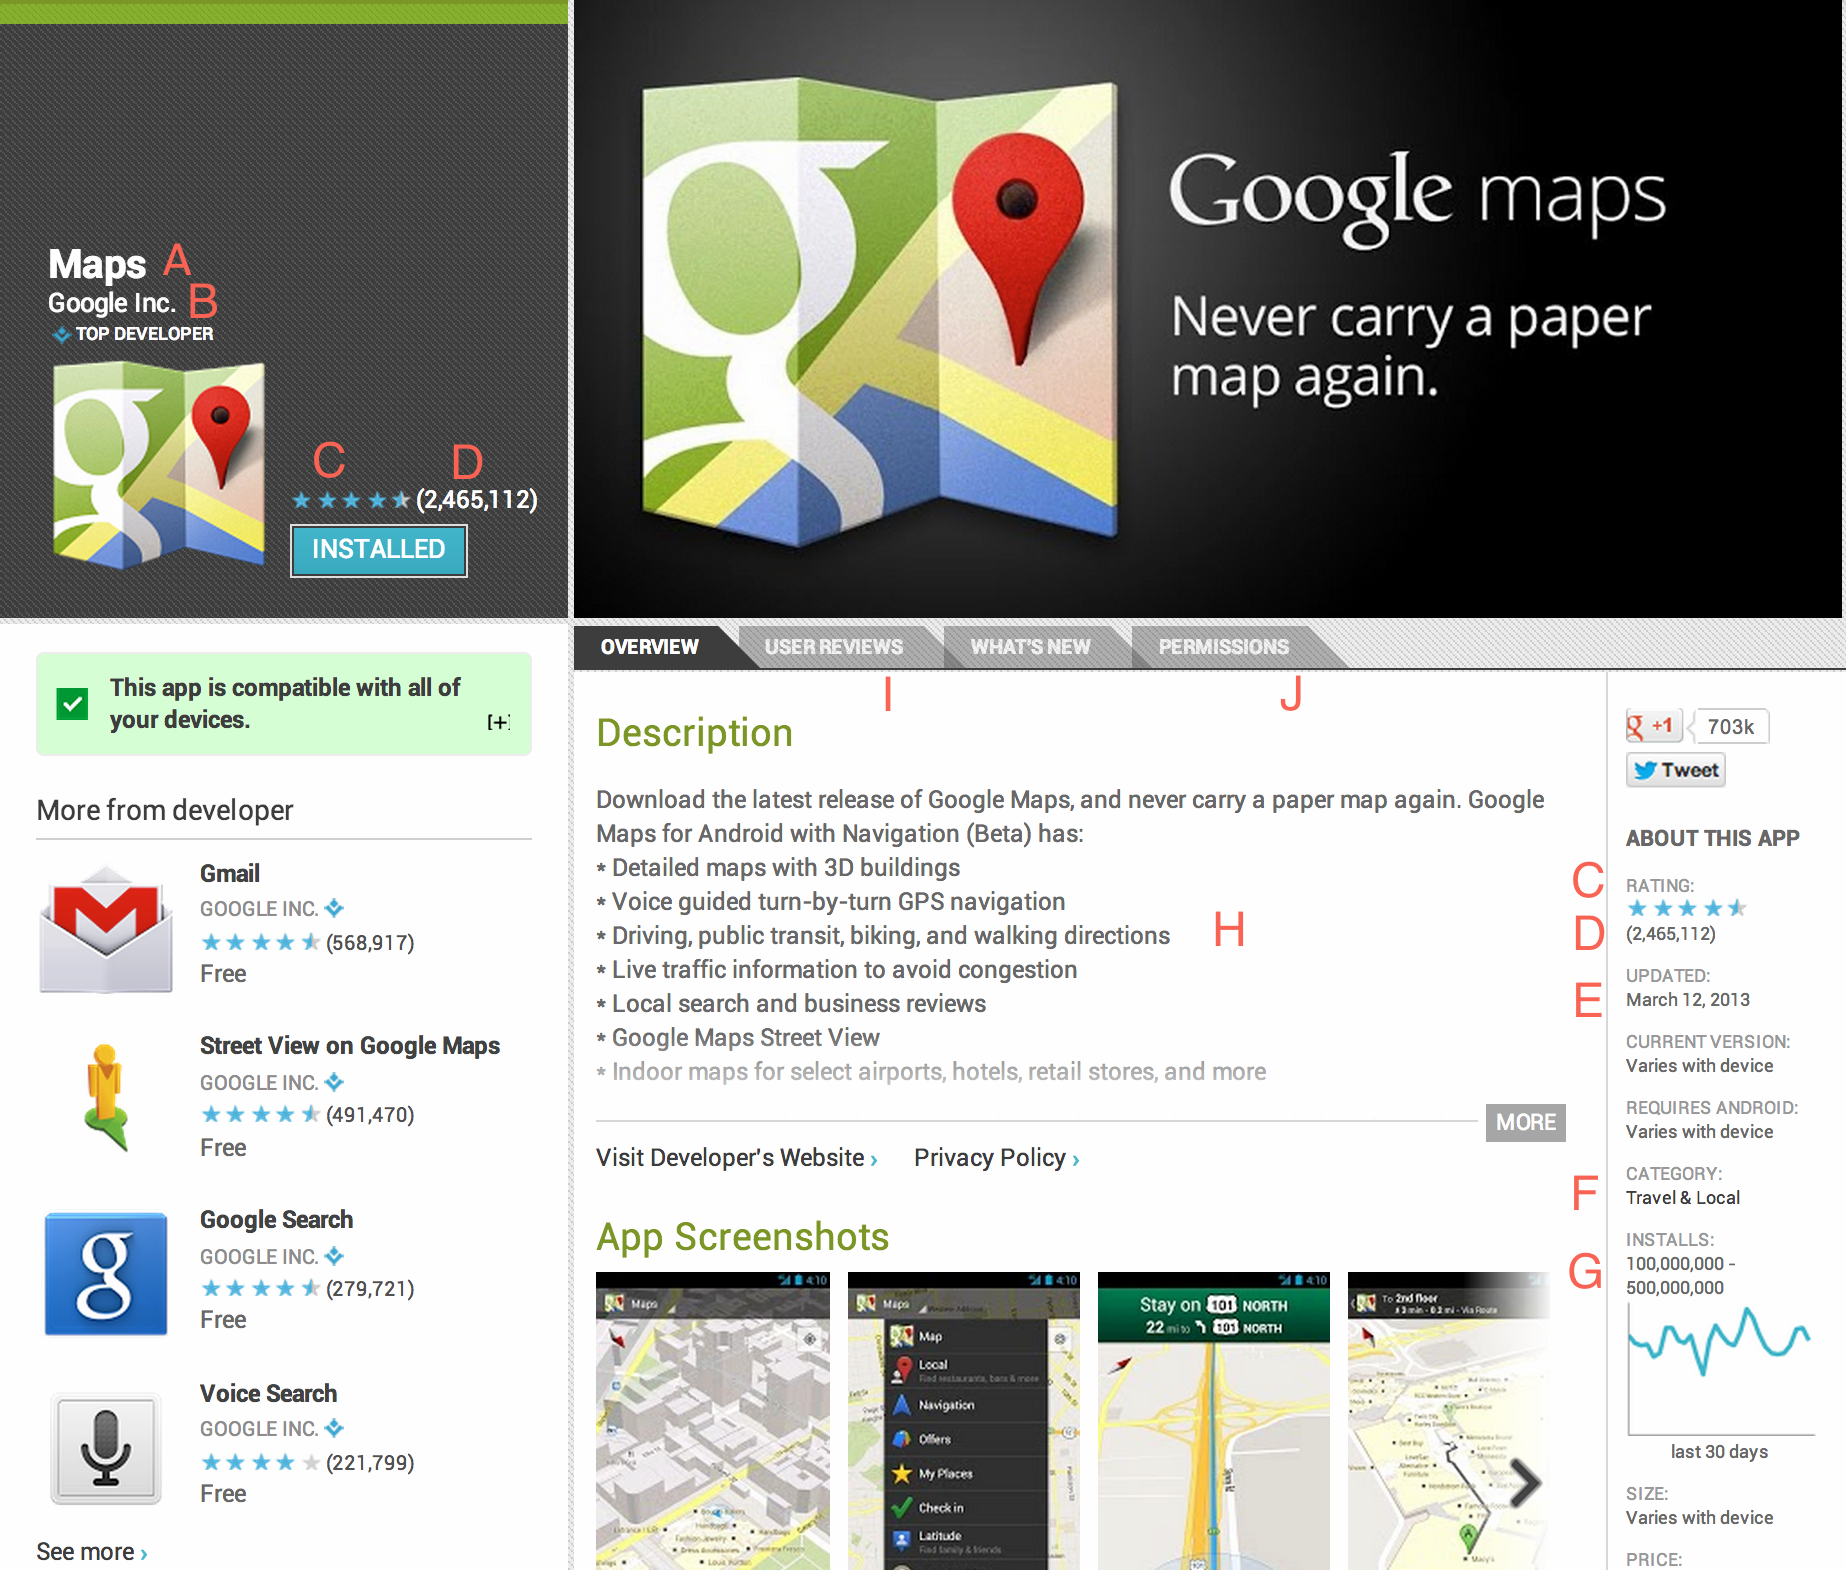
\includegraphics[width=0.9\columnwidth]{figs/GPStoreAppPage}
\caption{A sample page on the Google Play Store, see \ref{tab:gpstorekey}}
\label{fig:gpstoreapps}
\end{center}
\end{figure}

\begin{table*}[h]
\begin{small}
\begin{tabular}{l|l}

\textit{A} & App name  \\
\textit{B} & Developer Name  \\
\textit{C} & App Rating  \\
\textit{D} & Number of ratings  \\
\textit{E} & Date the app was last updated  \\
\textit{F} & Category in the Google Play Store it falls under  \\
\textit{G} & Number of installs (range, not exact number)  \\
\textit{H} & Description of the app  \\
\textit{I} & Reviews of the app  \\
\textit{J} & Permissions the app requests  \\

\end{tabular}
\end{small}
%\vspace{-0.2in}
\caption{Various properties of a Google Play Store app page}
\label{tab:gpstorekey}
%\vspace{-0.1in}
\end{table*}

%The core concept behind Android security - Permissions - are a static contract of capabilities. However, in this paper we propose an alternate means of conceptualizing security, which focuses on the interrelationship between the user's perception of the app, and the app's actual behavior. We call this the ``user-app agreement'', and will elaborate on it more later. 

\section{Malware}
Malware, as defined by the US Department of Homeland Security, is ``Short for malicious software. Programming (code, scripts, active content, and other software) designed to disrupt or deny operation, gather information that leads to loss of privacy or exploitation, gain unauthorized access to system resources, and other abusive behavior'' \citep{nash2005undirected}. Like PC OSs, malware is present on mobile OSs, although there are differences.


\subsection{Mobile Malware}
The tighter security model of Mobile OSs has a notable effect on mobile malware. With tight control in sandboxing, and app distribution, the usual viruses, trojans, and other exploits are more difficult to employ. The main vectors are either OS-level exploits, sneaking past the app review process, or through sideloading of apps. When looking at the two main mobile OSs, a stark contrast is shown. iOS has had  ``jailbreaking'' - privilege escalation exploits - dating back from it's first release \citep{damopoulos2011isam}, whereas the first Android exploit was not discussed until 2010 by security researchers Papathanasiou and Percoco \citep{papathanasiou2010not}, and was not seen in the wild until early 2011\citep{castillo2010android}. On the contrary, no side-loading is possible for iOS, and there have been very few - if any - instances of malware sneaking past Apple's App Store review process, although it has happened\footnote{In July 2012, SecureList noticed an iOS app that uploaded all of the user's contacts to a remote location without their consent\citep{SecureList2012}, but others argued this was not as devious as made out to be\citep{trendmicroios2012} }. With 95\% of all mobile malware\citep{nq2013}, Android's malware situation is very much a product of the sideloading and lack of review process found in GPStore\citep{nq2013}. %Of all the mobile malware found for iOS and Android, over \temp{some percent} used no system-exploits at all, \temp{some percent} on the main app distribution platform.

 On mobile devices, one of the dominant goals of malware is to gather information that leads to loss of privacy, found in over 28\% of mobile malware in 2012 alone\citep{nq2013}. This trend, of malware that possesses no system exploits, but gathers information that leads to loss of privacy, known as Info Theft Malware, is one that Android's Permission-based security model is ill-equipped to handle. Android's permission system relies on the user to determine at install-time if a list of capabilities should be entrusted with the given app. The user is not given a say in how or when the capabilities may be used, nor the ability to reject specific capabilities. At the same time, the mechanisms that keep mobile OSs safe are forcing malware writers to use more subtle techniques, often times without exploits. This all works against the user.

In this paper, we attempt to address this key issue through various means. We first introduce several novel concepts for analyzing apps and malware on Android. We then analyze the state of Android apps and Permissions with the most comprehensive android app database available, Android Census. Finally, we propose several novel improvements to the Android security architecture, called AndroMEDA, aimed at building off of our conceptual work.


\chapter{Permissions \& Security on Android}
\label{sec:permissions}

\begin{figure}[t]
\begin{center}
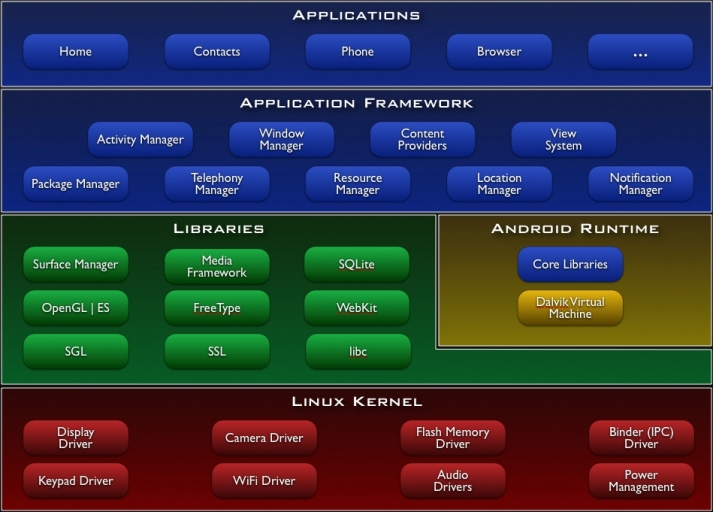
\includegraphics[width=0.7\columnwidth]{figs/system-architecture}
\caption{An overview of the Android system architecture, from \citep{androidarchitectureoverview}}
\label{fig:androidoverview}
\end{center}
\end{figure}


\section{Android Architecture Overview}
Android is an open-source project, built on Linux. Designed to be a lightweight, modular, extendable, and versatile operating system, Android removed almost all of the typical GNU/Linux stack, and wrote an entire framework from scratch. Built in Java, Android runs the Dalivk VM, a lightweight Java-compatible VM (see Figure \ref{fig:androidoverview}). 

The three major application components of Android are Activities, Services, and Content Providers. They are joined together through the Intent system. Activities are user-facing tasks, and follow the iOS definition of an ``app''. Only one may run at a time, and they have strict lifecycles. Services run in the background and follow a less strict lifecycle. Their main purpose is to perform long-running tasks that do not require user input. Lastly, Content Providers ``manage access to a structured set of data. They encapsulate the data, and provide mechanisms for defining data security. Content providers are the standard interface that connects data in one process with code running in another process''\citep{androidcontentproviders}.

Android was built from the ground-up to be composed of strongly isolated modules with little dependencies. No traditional SysV IPC is allowed; instead Android provides its own inter-app communication built off of its Intent system. Intents on Android, as described in the documentation, are ``an abstract description of an operation to be performed... An Intent provides a facility for performing late runtime binding between the code in different applications. Its most significant use is in the launching of activities, where it can be thought of as the glue between activities. It is basically a passive data structure holding an abstract description of an action to be performed''\citep{androidintents}. Intents allow apps to describe the operation they would like to perform, without explicitly identifying a recipient. For example, when the intent \textit{ACTION\_VIEW} is sent with data ``http://google.com'', Android searches through all installed apps that designate that they respond to that intent and will pick one to deliver it to; in this case, the \textit{Browser} would respond.

\section{Android Permissions}
The highly modular and decentralized aspect of Android makes it extremely easy to tap into virtually all Personally Identifiable Information on the device. To protect this, and many other aspects of the system, Android utilizes the Permission security model. The permission security model is a static list of capabilities an app possesses: when presented with this list before installation (see Figure \ref{fig:gpstorepermissions}), a user will either grant the app access to the features or simply not install the app. When an app requests a permission, the Android system treats it as if the user granted the app that capability. After installation, this list will never change unless the app package itself changes and the user reviews the new permissions.

\begin{figure}[h]
\begin{center}
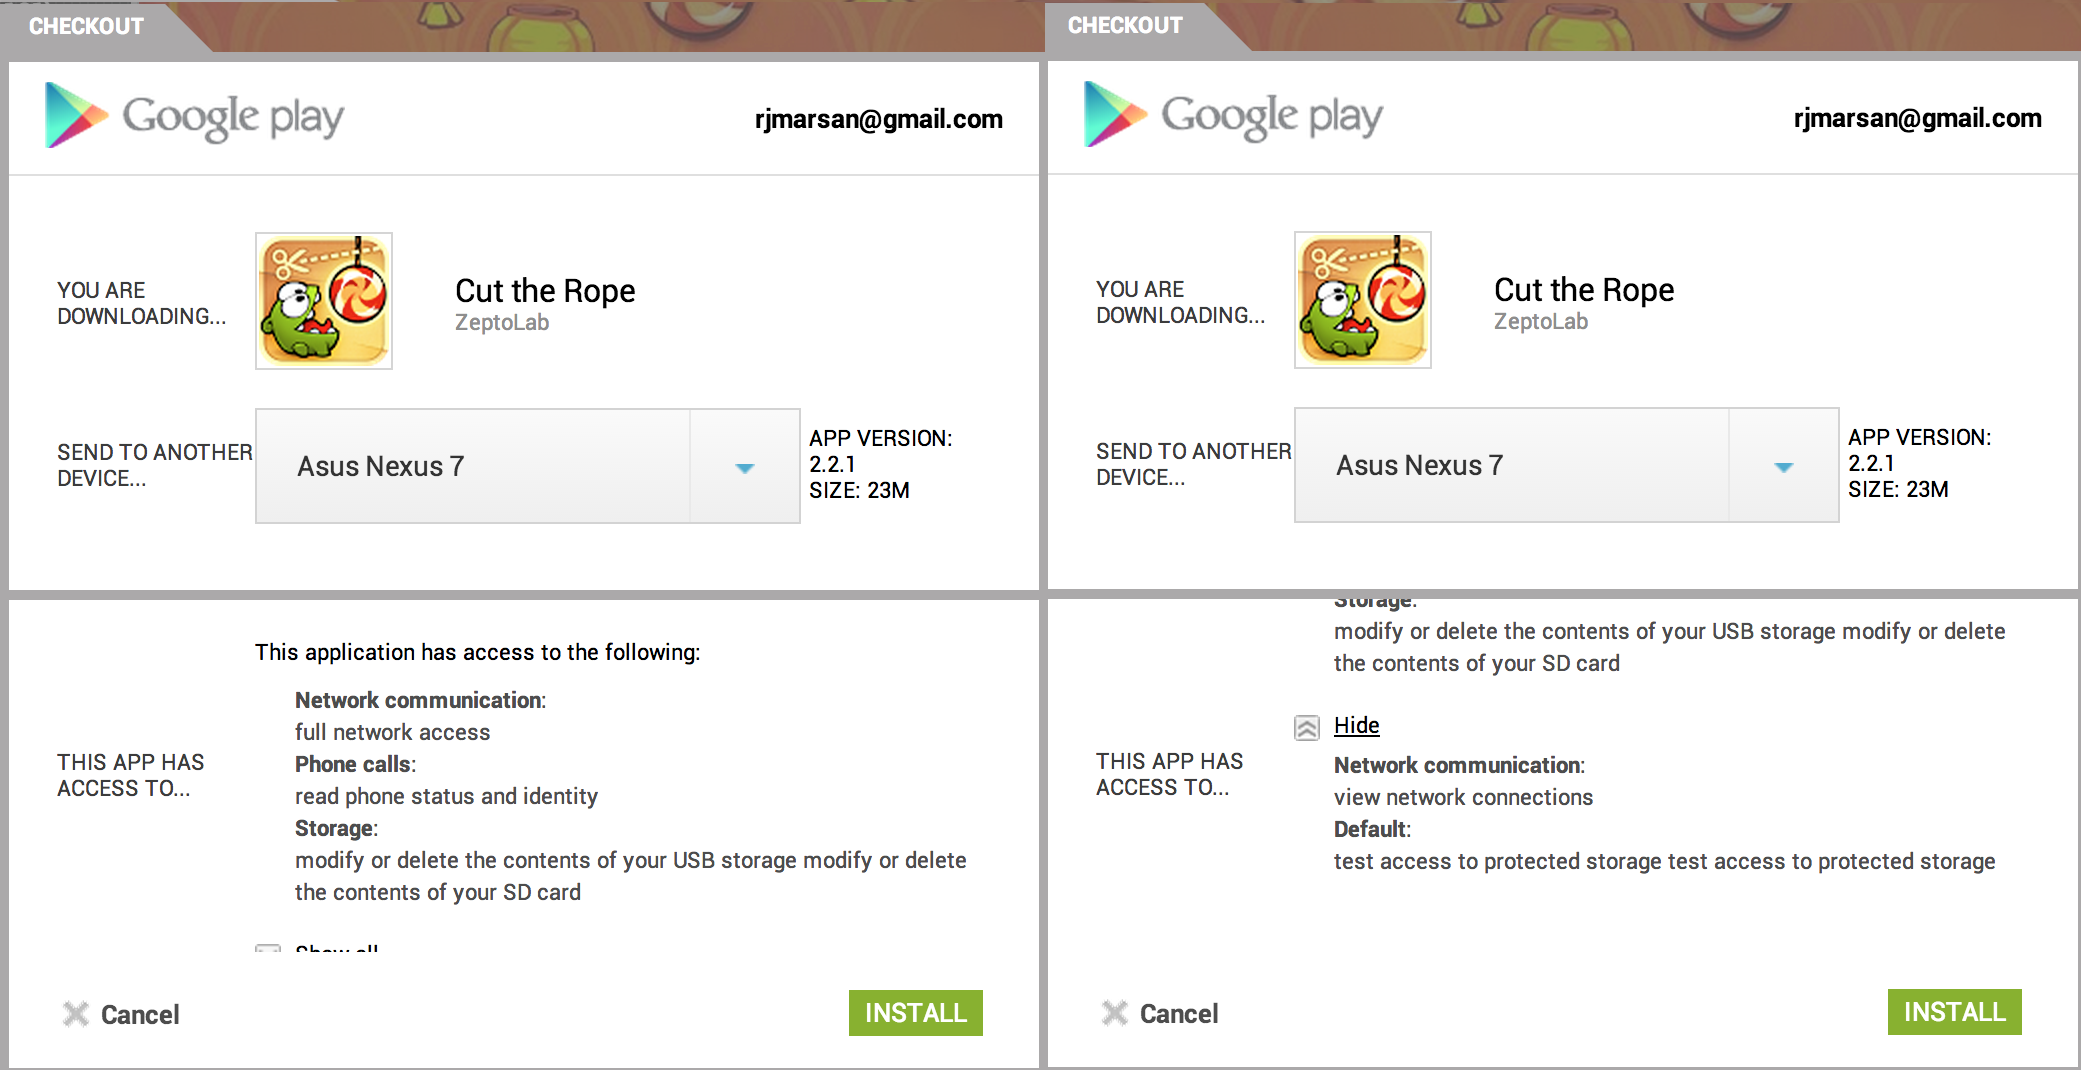
\includegraphics[width=1.0\columnwidth]{figs/GPStoreInstallScreen}
\caption{A sample Google Play Store install screen showing the permissions. The user must scroll to see all of them, and click ``Show All'' to see the hidden ones.}
\label{fig:gpstorepermissions}
\end{center}
\end{figure}

Android permissions themselves are much more granular than a typical UNIX permission system. They cover a wide variety of operations, including controlling the sleep state, accessing hardware, accessing PII, and many system operations. Some of the most requested permissions can be seen in Table \ref{tab:perms}; the rest can be seen in Appendix Table \ref{tab:allperms}.

%\begin{smitemize}
%\item \textit{android.permission.INTERNET}: Grants the app access to network sockets. Without this, an app alone could not access the internet over WiFi, 3G, or other interfaces. No restrictions are placed on the protocol, ports, or domains accessed.
%\item \textit{android.permission.WAKE\_LOCK}: Prevents the device from sleeping. When a Wake Lock is acquired, the Android system will not shut off. Depending the Wake Lock, the screen may continue to stay on, or it may turn off, but the CPU and other hardware remains in operation.
%\item \textit{android.permission.READ\_PHONE\_STATE}: Grants the app access to the phone hardware, which includes IMEI, GSM information, as well as the phone number of the current call. Since the IMEI is frequently used as a UDID, this is a popular permission.
%\item \textit{android.permission.CAMERA}: Allows apps access to the camera hardware, if present. The Android system still requires an app hold a valid drawing surface before data is sent to the app, making it difficult to perform in the background.
%\item \textit{android.permission.READ\_CONTACTS/READ\_SMS/READ\_CALENDAR}: offers read-only access to personal information. <say more?>
%\item \textit{android.permission.WRITE\_CONTACTS/WRITE\_SMS/WRITE\_CALENDAR}: offers write-only access to personal information. <say more?>
%\end{smitemize}





\begin{table*}[t]
\begin{small}
\begin{tabular}{p{3cm}|p{12.5cm}}
Permission  & Description \\
\hline

\textit{INTERNET} & Network communication. full Internet access. Allows the app to create network sockets.  \\
\textit{WRITE\_EXTERNAL\_\-STORAGE} & Storage. modify/delete USB storage contents modify/delete SD card contents. Allows the app to write to the USB storage.  Allows the app to write to the SD card.  \\
\textit{READ\_PHONE\_STATE} & Phone calls. read phone state and identity. Allows the app to access the phone features of the device.  An app with this permission can determine the phone number and serial number of this phone, whether a call is active, the number that call is connected to and the like.  \\
\textit{ACCESS\_FINE\_\-LOCATION} & Your location. fine (GPS) location. Access fine location sources such as the Global Positioning System on the tablet, where available.  Malicious apps may use this to determine where you are, and may consume additional battery power.  \\
\textit{ACCESS\_COARSE\_\-LOCATION} & Your location. coarse (network-based) location. Access coarse location sources such as the cellular network database to determine an approximate tablet location, where available.  Malicious apps may use this to determine approximately where you are. \\
\textit{WAKE\_LOCK} & System tools. prevent tablet from sleeping prevent phone from sleeping. \\
\textit{READ\_CONTACTS} & Your personal information. read contact data. Allows the app to read all of the contact (address) data stored on your tablet.  Malicious apps may use this to send your data to other people. \\
\textit{CALL\_PHONE} & Services that cost you money. directly call phone numbers. Allows the app to call phone numbers without your intervention.  Malicious apps may cause unexpected calls on your phone bill.  Note that this doesn't allow the app to call emergency numbers.  \\
\textit{CAMERA} & Hardware controls. take pictures and videos. Allows the app to take pictures and videos with the camera.  This allows the app at any time to collect images the camera is seeing.  \\
\textit{WRITE\_CONTACTS} & Your personal information. write contact data. Allows the app to modify the contact (address) data stored on your tablet.  Malicious apps may use this to erase or modify your contact data.  \\
\textit{GET\_TASKS} & System tools. retrieve running apps. Allows the app to retrieve information about currently and recently running tasks.  Malicious apps may discover private information about other apps.  \\
%\textit{WRITE\_SETTINGS} & System tools. modify global system settings. Allows the app to modify the system's settings data.  Malicious apps may corrupt your system's configuration.  \\
\textit{RECORD\_AUDIO} & Hardware controls. record audio. Allows the app to access the audio record path.  \\
\textit{SEND\_SMS} & Services that cost you money. send SMS messages. Allows the app to send SMS messages.  Malicious apps may cost you money by sending messages without your confirmation.  \\
\textit{READ\_HISTORY\_\-BOOKMARKS} & Your personal information. read Browser's history and bookmarks. Allows the app to read all the URLs that the Browser has visited, and all of the Browser's bookmarks.  \\
\textit{READ\_CALENDAR} & Your personal information. read calendar events plus confidential information. Allows the app to read all calendar events stored on your tablet, including those of friends or coworkers.  Malicious apps may extract personal information from these calendars without the owners' knowledge. \\
\textit{WRITE\_HISTORY\_\-BOOKMARKS} & Your personal information. write Browser's history and bookmarks. Allows the app to modify the Browser's history or bookmarks stored on your tablet.  Malicious apps may use this to erase or modify your Browser's data \\
\textit{RECEIVE\_SMS} & Your messages. receive SMS. Allows the app to receive and process SMS messages.  Malicious apps may monitor your messages or delete them without showing them to you.  \\
\textit{WRITE\_CALENDAR} & Your personal information. add or modify calendar events and send email to guests without owners' knowledge. Allows the app to send event invitations as the calendar owner and add, remove, change events that you can modify on your device, including those of friends or co-workers.  Malicious apps may send spam emails that appear to come from calendar owners, modify events without the owners' knowledge, or add fake events.  \\
%\textit{CHANGE\_WIFI\_STATE} & System tools. change Wi-Fi state. Allows the app to connect to and disconnect from Wi-Fi access points, and to make changes to configured Wi-Fi networks.  \\
%\textit{ACCESS\_MOCK\_LOCATION} & Your location. mock location sources for testing. Allows the app to create mock location sources for testing.  Malicious apps may use this to override the location and/or status returned by real location sources such as GPS or network providers.  \\
%\textit{PROCESS\_OUTGOING\_CALLS} & Phone calls. intercept outgoing calls. Allows the app to process outgoing calls and change the number to be dialed.  Malicious apps may monitor, redirect, or prevent outgoing calls.  \\
%\textit{MODIFY\_AUDIO\_SETTINGS} & Hardware controls. change your audio settings. Allows the app to modify global audio settings such as volume and routing.  \\
\textit{MOUNT\_UNMOUNT\_\-FILESYSTEMS} & System tools. mount and unmount filesystems. Allows the app to mount and unmount filesystems for removable storage.  \\
\textit{READ\_SMS} & Your messages. read SMS or MMS. Allows the app to read SMS messages stored on your tablet or SIM card.  Malicious apps may read your confidential messages. \\
\textit{READ\_LOGS} & Your personal information. read sensitive log data. Allows the app to read from the system's various log files.  This allows it to discover general information about what you are doing with the tablet, potentially including personal or private information.  \\
\textit{DISABLE\_KEYGUARD} & System tools. disable keylock. Allows the app to disable the keylock and any associated password security.  A legitimate example of this is the phone disabling the keylock when receiving an incoming phone call, then re-enabling the keylock when the call is finished.  \\
%\textit{BLUETOOTH} & Network communication. create Bluetooth connections. Allows the app to view the configuration of the local Bluetooth tablet, and to make and accept connections with paired devices. \\
%\textit{WRITE\_SMS} & Your messages. edit SMS or MMS. Allows the app to write to SMS messages stored on your tablet or SIM card.  Malicious apps may delete your messages. \\
%\textit{CHANGE\_CONFIGURATION} & System tools. change your UI settings. Allows the app to change the current configuration, such as the locale or overall font size.  \\

\end{tabular}
\end{small}
%\vspace{-0.2in}
\caption{Frequently Requested Android permissions, and the GPStore's description of them}
\label{tab:perms}
%\vspace{-0.1in}
\end{table*}





In cases like \textit{WAKE\_LOCK} and \textit{CAMERA}, the permission seems fairly singular: access to exactly one feature. However, for other permissions, such as \textit{INTERNET} and \textit{READ\_PHONE\_STATE}, many more granularities could be established. For example, \textit{INTERNET} gives unconditional access to all domains, unlike web pages in modern web browsers. In addition, while permissions are intended to be non-overlapping, there still are ways --- varying from minor to major --- to acquire information guarded by one permission from another. For example, \textit{READ\_PHONE\_STATE} can access to the current phone call, and is able to establish call logs, an operation normally protected by \textit{READ\_CONTACTS}. There are some permissions, however, that are explicitly supersets of another other, such as \textit{ACCESS\_COURSE\_LOCATION} --- providing network-tower location --- and its superset, \textit{ACCESS\_FINE\_LOCATION} --- providing GPS location. 

Permissions do not tend to change through Android's release history. As new hardware is made accessible through Android's SDK, new permissions are added for them, but there are very few times when permissions drastically change meaning or scope. Through Android's 6 year history, only 3 new permissions has been added to restrict previously unrestricted operations\footnote{In Android 4.1, the storage device requires a permission to read, and the call logs require a separate permission to read and write --- previously they shared a permission with contacts\citep{android41new}.}.

\section{Permission Enforcement}
Permission enforcement on Android is generally performed in two main ways: UNIX permissions and explicit runtime checking. Most hardware is accessible using C or other low-level calls, so permissions are more effectively enforced via UNIX Group Permissions. Upon app installation, Android assigns each app a unique UID and assigns different group permissions to that user. For example, socket access is granted to a UNIX group, and all apps that request \textit{INTERNET} are added to that group. This is simple, effective, and has very little performance overhead. Unfortunately, it makes it difficult to put any additional enforcements as to when and how these resources are accessed. 

System operations, like wake locks, changing system settings, turning on and off components, is checked on every API call, through a centralized PackageManager class. The PackageManager first checks if the app has requested that permission. If it has, it then proceeds to check if the permission is protected by the system. Some permissions are only available to trusted code, through either a shared key, or being located in a system folder. Many system operations fall into this category, including \textit{WIPE\_DEVICE}, and \textit{BRICK}. These operations typically are extremely dangerous, and have the potential to destroy a device, or perform elaborate phishing operations. Even if an app requests the permission, the PackageManager still has the right to reject the operation. This allows system-level operations to be exposed to trusted developers post-deployment on a device, while still protecting the operations from untrusted developers.

The final aspect of permissions deal with protecting PII. Android implements the bulk of PII sources through Content Providers, which sit in front of a dataset and provide access to remote services. It is therefore imperative for each individual data source to check the permissions of the incoming app, every time it is requested. This, however, provides opportunities to extend on its behavior.

\subsection{Permission Rejection}
\label{sec:permissionrejection}
When a permission is checked on Android, one of two outcomes is possible. The check passes, and the operation continues as intended, or the check fails, and an exception is thrown. By design, the code path instantly jumps to an error state, halting the action. No logging of this action takes place, nor are partial passes allowed.

\section{Third Party Permissions}
\begin{sloppypar}
Android was built to distribute PII in a modular fashion, and it extended these features to other third party apps. Any developer may write Content Providers, and likewise, can create Permissions to protect them. Other apps must request that permission before accessing the data. An example of this: Alice writes a messaging app, \textit{MyMessenger}. She wants to expose the PII to other apps, so she makes a Content Provider around it. To protect the user's information, she defines her own permissions: \textit{mypackage.MyMessenger.READ\_MESSAGES} and \textit{mypackage.MyMessenger.WRITE\_MESSAGES}. Bob writes an app that uses \textit{MyMessenger}'s data to build a picture. His app requests the permission \textit{mypackage.MyMessenger.READ\_MESSAGES}. When his app contacts Alice's Content Provider, she checks this custom permission before proceeding with the query. However, if Bob does not request \textit{mypackage.MyMessenger.WRITE\_MESSAGES} and attempts to perform a write action, Alice's Content Provider will reject the operation.
\end{sloppypar}
%These rejections are not logged or notified. expand on this.


If two apps request the same permissions, as long as neither have access to system permissions, it can be assumed that they have the same capabilities. These capabilities are permanent as well, as permissions for a given package can not be added nor removed. This Permission Fingerprint, or set of capabilities, uniquely defines what an app has access to. All apps that request the same set of permissions have access to the exact same set of actions, and only through those permissions do they have those actions (with a few exceptions). However, Android permissions are static, therefore a Permission Fingerprint doesn't guarantee a specific pattern of behavior. In fact, since not all permissions are guaranteed to be granted, a Permission Fingerprint simply establishes the absolute maximum capabilities of an app - even if the system rejects some of them.

\chapter{Malware on Android}
\label{sec:malware}

Malware on mobile devices has seen a departure from past exploits. The wealth of Personally Identifiable Information easily available on mobile OSs increasingly makes them the focus of malicious software. In addition, the tight sandboxing constraints often forces malware writers to either find exploits to break out of the sandbox or to write malware that cloaks itself as benign. Without finding exploits, code can not be run by the user unless it is in it is form and comes through a trusted channel (unless of course that security feature has been disabled). Once on the device, malware has several main methods of attack.

\section{Installation}
The three primary ways in which malware can be installed on an Android device are \textit{Repackaging}, \textit{Update Attack}, and \textit{Drive-by Download}\citep{zhou2012dissecting}. The first two are designed to sneak malware into the Google Play Store or other third party stores; and the third is designed to trick the user into installing it by mistake. \textit{Repackaging} deals with the technique of taking an existing app, adding malicious code to it, and repackaging it again (discussed further in Chapter \ref{sec:incognitoware}). \textit{Update Attacks} typically build off of \textit{Repackaging}, but do not acquire malicious code until later, making static detection difficult\citep{zhou2012dissecting}. The last, \textit{Drive-By Downloads}, is often tied with \textit{Repackaging}, but is not presented in an official app channel. Instead, it is downloaded when the user visits a webpage or clicks a link\citep{zhou2012dissecting} and Android prompts the user as to whether or not they would like to install the app. All three methods involve concealing the intent of the malware and passing as a legitimate app; they do not use browser exploits or system exploits to install the initial malware without the user's consent.

\section{Malicious Actions}
Once installed on the device, Android malware has several main methods of attack. Xuxian Jiang
 and Yajin Zhou\citep{zhou2012dissecting}, along with Spreitzenbarth\citep{spreitzenbarth2013}, and Hackmageddon\citep{hackmageddon2011} define four major categories: \textit{Privilege Escalation Attack}, \textit{Remote Control Attack}, \textit{Monetary Service Attacks}, and \textit{Privacy Info Theft}. 


\section{Privilege Escalation Attack}
\textit{Privilege escalation attacks} take several forms on Android. The basic premise is simple: acquire access to operations beyond what the sandbox and granted capabilities provide. The main way to accomplish this is via \textit{rooting}.

\subsection{Rooting}
\textit{Rooting} is the act of acquiring root --- or administrative privileges --- on an OS. Typically mobile OSs do not provide the user or apps with root capabilities and instead reserve that for a set of trusted system processes. However, by finding vulnerabilities in these services or exploiting the OS itself, apps can escape the sandbox. After an app has been granted root capabilities, the permission system no longer applies to it: it can simply access whatever it wants. These attacks are difficult for the system to detect as all monitoring of apps relies on monitoring the sandbox --- there is no way to track an app that escapes the sandbox. This technique is commonly employed by botnets, giving remote access to the core system. 

Many examples of root exploits exist, dating back to 2011 with \textit{RageAgainstTheCage}\citep{droiddream}. These root exploits were very popular for non-malicious purposes, circumventing the device's sandbox to install a permanent root binary, creating a similar setup to a typical UNIX computer, where root may be acquired after a password and/or permission. In March 2011, however, DroidDream was discovered. DroidDream used \textit{RageAgainstTheCage} to silently install additional applications in the background, stealing PII and forming a botnet. By the time Google remotely removed it from the market, it had been downloaded an estimated 50,000 to 200,000 times\citep{castillo2010android}, which was the largest bulk-remote-removal of apps seen from the GPStore. From then on, a stream of root exploit malware was found based off of exploits such as \textit{RageAgainstTheCage}, \textit{udev}, and another called \textit{GingerMaster}\citep{gingermaster}.

\subsubsection{Recent Android Rootkits}
\label{sec:recentrootkits}
\textit{GingerMaster}\citep{cskills2011} is significant because it is the last known root exploit malware seen in use. Designed for Android 2.3.3, it can currently run on 45\% of all Android devices in use, according to the official Android Dashboard\citep{androiddashboard}. In reality, however, of that 45\%, almost all have been patched to fix the exploit\citep{cskills2011}. All previous exploits were patched in Android 2.3\citep{cskills2011}, meaning less than 6\% of all active Android devices are vulnerable to them. Since Android 4.0, Google has focused greatly on security, improving ASLR\citep{threatpost2012} and hardening system services\citep{androidjbsecurity}. No known rootkits exist --- malicious or not --- for Android 4.0 and up comprising 54\% of active Android devices.

 %Several exploits became very popular for malware writers, starting with DroidDream in 2010 <cite>, then RageAgainstTheCage, PSNeuter, and GingerBreak. When DroidDream was first discovered, it was downloaded over <50,000> times in the GPStore - prompting the largest bulk-remote-removal of apps Google has ever been discovered to have performed. However, most of these attacks have been fixed by vendors as of Android 2.3.3 - meaning the total amount of current devices in use that are vulnerable to these bugs being roughly <10%>. After these attacks, Android has taken definite steps to up its security. Since 4.0, proper ASLR has been implemented, as well as other security enhancements. There has been no known malware written for Android 4.0 and up - over <50%> of the active market.

\subsection{Confused Deputy Attack}
The second main vector for privilege escalation attacks is the \textit{confused deputy attack}\citep{hardy1988confused}. In this scenario, services that guard sensitive operations are ``tricked'' into performing them. For example, if a Content Provider forgets to check a permission, or if a developer finds APIs that do not correctly perform a permission check. Perhaps the simplest example of this is the ability for any Android app to contact remote servers by asking the web browser to open a URL. By including sensitive data in the URL, an app may still transmit sensitive data to a remote server without ever requesting the \textit{INTERNET} permission. Projects like XManDroid\citep{bugiel2011xmandroid} and Quire\citep{dietz2011quire} address this by extending Android to analyze inter-app communication and detect this kind of attack. %Despite all of these concerns, it is worth noting that no known malware has been used to exploit this. 

\section{Remote Control Attack}
\textit{Remote Control Attacks}, frequently called \textit{botnets}, are the ability for malware to accept commands from a remote server, controlling the device. This technique is common --- Xuxian Jiang
 and Yajin Zhou\citep{zhou2012dissecting} found in 93\% of Android malware --- and is often used in conjunction with other attacks\citep{spreitzenbarth2013}.

\section{Monetary Service Attack}
\label{sec:premiumsms}
The second malware technique is possibly the simplest: perform services on behalf of the user that cost money. Examples of this include calling costly phone numbers and sending premium SMS messages. Typically these actions are performed without notifying the user, and are only visible after the user checks their bill. These attacks have been prevalent in the Android market for quite a while, with NQ Mobile\citep{nq2013} listing it as one of the top three threats of 2012, and being found in 39 of 119 of the malware documented by Spreitzenbarth\citep{spreitzenbarth2013}. However, recent versions of Android (after 4.2 Jelly Bean\citep{androidjbsecurity}) have taken the step of warning the user before premium SMSs are sent. %This attack vector, while common, will see a reduction in the future thanks to these measures.

A prime example of this is FakeInst\citep{avastfakeinst}, a repackaged version of Instagram\citep{instagramandroid} that sent premium SMS messages on start. ``In the background, the fake downloader sends a premium rate SMS to the number based on the country of origin for the user''\citep{avastfakeinst}. In many cases, the premium SMS messages would end up being billed to the user for over \$4 each\citep{avastfakeinst}, without ever alerting the user. Messages are often deleted by the app, removing the trace until the user gets their bill.
%\temp{Expand on this more}
%show some examples of this. expand on this more.

\section{Private Info Theft}
The last malware technique is the most significant, and represents the largest departure from typical malware: apps that steal PII, or \textit{Info Theft Malware}. The theme is fairly straightforward: provide the user with a seemingly legitimate app, but in the background acquire large amounts of valuable data --- including call logs, contacts, and photos --- and send them to a remote server. This fits with the main themes of mobile computing: the consolidation of many sources of PII all in one device. 
%However, this is the biggest departure from typical malware. 
To the system no unusual operations are performed and no exploits are ran. The qualification for Info Theft Malware lies in the ``use'' vs ``misuse'' of PII; often times, this line is blurred.

\subsection{Path on iOS}
\label{sec:path}
A large distinction of what constitutes as privacy malware to an individual stems from the user's expectations of how the app will use their PII. Consider the case of the Path iPhone app, which in February 2012 was discovered to be uploading the user's entire contact list to Path's servers, without any consent from the user\citep{thampi2012}. It is fairly uncontroversial for a social network to read your contact data, and the act of scanning contacts to help ``find your friends'' on Path wasn't out of the ordinary. As VentureBeat discovered: ``Facebook, Twitter, Instagram, Foursquare, Foodspotting, Yelp, and Gowalla are among a smattering of iOS applications that have been sending the actual names, email addresses and/or phone numbers from your device's internal address book to their servers''\citep{vb2012addressbook}. Ultimately, however, the outrage was sparked because of how unexpected the behavior was.

The Path incident sparked several key changes in iOS's security model: having a popup occur when an app requests access to the contacts database and allowing the user to reject the request. This, in general, is a one-time request, after which the app is granted unrestricted access to the content\citep{AppleContacts}. This change, however, did not fully address situations like Path, in which is was less about the app simply having access to the data, and more about what the app actually did with the data behind the scenes. When these actions did not match up with user expectations, it was treated as malware until the situation was cleared up by Path. The next day, they issued an update immediately explaining to the user what they were going to do with the data, and why.

It is worth noting that the only reason Path's contacts upload mechanism was discovered was by accident: Arun Thampi discovered it as part of a company hackathon, and only via sniffing the HTTP requests coming from the phone. An ordinary smartphone user would not have access to these tools, nor have the time and patience to sift through the data to spot unusual behavior. These actions are unchecked and hidden from the user, not giving them a chance to decide for themselves if they are comfortable with them - supporting our motivation for AndroMEDA.

\section{User-App Agreement}
This incident, however, lies at the heart of mobile malware: Misuse of PII lies in the abstract definition of how the app is expected to behave. Apps that violate this expectation of behavior are classified as malware, and apps that do not are not. This agreement between the user and the app, the User-App Agreement (or UAA), is an informal understanding the user has as to what actions an app will take. This differs from the Permission Fingerprint, which is a measure of what actions the app is capable of performing, instead dealing with exactly when and how those actions are taken. Since this agreement is not formally defined, it is acquired through external trust in an app. This happens in various ways, through the description the app provides, to the knowledge and referral of the app from other trusted sources, or the trust in the developer. The UAA is not a measure of how trustworthy an app is, but rather a framework for the user consenting and trusting specific actions an app may take.

\subsection{UAA Example - Social Networking App}
An example of UAA can be seen in the expected behavior of a hypothetical app and user. The first is a large Social Networking app, which requests permission to access internet, send SMS messages and read the contacts database. If the Social Networking app accesses contacts when the user requests it ``find my friends'', and it sends SMS messages after the user messages another user who is not ``online'', these actions fall within the UAA of the Social Networking app and the user. However, if the contacts database is read and uploaded to a remote server without the consent of the user, this may violate the UAA, breaking the trust of the user (building off the example of Path). 

\subsection{UAA Example - Social Game}
The other example is a little known developer's game, which also requests permission to access internet, send SMS messages and read contacts, same as the Social Networking app. These documented capabilities in the Permission Fingerprint may be enough to violate the UAA: the user may not trust an app with the capability of these actions. However, in the case that the user does, or simply doesn't pay attention, the app still may not violate the UAA. If the app is an online game, and asks you to find other people you know who are playing it, this would more likely than not violate the UAA. However, if it sends SMS messages to your friends telling them to download the game, this would breech the UAA, breaking the trust of the user.

In both examples, the apps have the exact same Permission Fingerprint, but vary wildly in their expected behavior, and which actions are trusted and untrusted. This fits right along with our definition of malware, with the misuse of PII and other device capabilities. This also highlights the shortcomings of the Permissions framework - being unable to deal with the subtle differences between trusted behavior and untrusted behavior. Indeed, for any given user, they may have a very different understanding of what acceptable behavior is. Therefore, UAA plays a crucial role in classifying apps in relation to Info Theft Malware.

\section{Proof of Concept Malware in Academia}
In the realm of malware research in academia, several prominent proof-of-concept examples further demonstrate the vague line between use and misuse of PII, and our concept, the User-App Agreement. The most notable one is SoundComber\citep{schlegel2011soundcomber} It passes off as a benign app, but in the background records audio, and does on-phone processing to find sensitive PII, after which it uploads the information to a remote server. This app is unique because of its simple Permission Fingerprint, and its ability to gather sensitive PII from a channel not suspected to be very rich in PII.

The second prominent example of academic malware on Android is TapLogger\citep{xu2012taplogger}. TapLogger imitates a simple touch-based game, learning the vibration patterns of the device for each tap. After which, TapLogger records the vibration patterns in the background, attempting to discover passwords and other sensitive keyboard events, all through a seemingly trusted sensor. TapLogger requests no Permissions, therefore its behavior is a possible behavior of virtually all apps. 

In Chapter \ref{sec:incognitoware}, we build upon these examples to present an additional dataset of research IncognitoWare, or repackaged apps with malicious software added. We keep the Permission Fingerprints identical to the cloned app, making detection exceptionally difficult. 
%reference future malware set

\section{Conclusion}
The landscape of malware on Android follows many clear patterns. The first is the use of masquerading as benign apps, and passing through trusted/semi-trusted channels to enter the device. Once on the device, the four main categories of attacks are privilege escalation attacks, remote control attacks, monetary service attacks, and info theft. Of these three attacks, privilege escalation and monetary service attacks are the easiest to protect against, and indeed Android has taken serious steps to mitigate these. However, the third time of attack, Info theft, is the most difficult to mitigate on Android, due to the shortcomings of the Permissions framework, and the wide spectrum of severity these attacks can take. Since these attacks may vary in interpretation per user, and lay in the subtle communication between the user and the app, we highlight the need for a concise representation UAA, where the user can evaluate the actions themselves.

\chapter{Related Works}
\label{sec:relatedworks}

%\temp{THIS WILL/MAY BE GREATLY EXPANDED UPON LATER}

\section{Android Extensions}
AndroMEDA is far from the first to attempt to address the issue of malware on Android. As early as 2009, frameworks like SAINT\citep{ongtang2012semantically} built off of the Android Permission Framework by implementing runtime policies the user could define per-app. Later on, projects like TISSA\citep{zhou2011taming} built off of SAINT by implementing varying levels of obfuscated data. When an app running on TISSA requests access to the contacts database, TISSA can either provide the app the full database, some limited portion, some anonymized portion, or outright returning no information. Not all PII was covered in their framework, nor were any temporal rules established: the system behavior for a specific database of PII for an app was consistent across requests. These events were not shown to the user either, something addressed by TaintDroid\citep{enck2010taintdroid}.

TaintDroid is a novel extension for Android, focused on flow detection of PII. By modifying the low level VM of Android, Dalvik, variables are tainted once they access PII. This taint flows throughout the system, and when the variable reaches a designated exit location, the event is logged and alerted to the user. Finally, YAASE\citep{russello2011yaase} is a relatively new security extension, but combines many aspects of TaintDroid and TISSA, to become an extremely powerful way of detecting information flow and prevention.

There are several main shortcomings in all of these frameworks. First off, they all require significant modification of the Android codebase, thus creating very difficult work for developers who seek to incorporate these extensions into their Android OS. Performance impact, although somewhat negligible by many accounts, certainly plays a role in a decision to incorporate such security extensions.

Another important shortcoming is the complex rulesets required. Most build off of the Permission Framework, adding additional rules the user may configure. However, a study by Berkeley suggests only 17\% paid attention to permissions at install time, and only 3\% correctly remembered them later\citep{felt2012android}. Clearly, tasking the user with more work is not the right approach. Looking at malware through the context of the UAA, all but TaintDroid fall short in one key regard: alerting the user of suspicious behavior.

Several frameworks have touched upon the concept of the UAA. Andromaly\citep{shabtai2012andromaly}, developed in 2010, pBMDS\citep{xie2010pbmds} and Crowdroid\citep{burguera2011crowdroid} all attempt to classify malware based upon its interaction with the user. However, none actually ask input from the user - a fundamental flaw that limits the ability to adapt to the user's specific UAAs.

\section{Android Sandboxes}
On the other side of malware detection is automated malware detection. The major project in this regard is Google's Bouncer\citep{googlebouncer}. Introduced in 2011, Google Bouncer is a system that runs malware in a highly-observed sandbox, and watches for suspicious behavior. Since its release, it has been the subject to quite a bit of criticism\citep{mansfield2012android}, with researchers finding over 20 ways to circumvent it.

Along similar lines, TrendMicro provides its solution, App Reputation\citep{trendmicroappreputation}. It runs apps in a ``cloud'' sandbox, watching for connections to suspicious websites, as well as other monitoring. A research project, Paranoid Android\citep{portokalidis2010paranoid}, runs in a similar vein, monitoring apps in a sandboxed Android OS. However, in order to get accurate information on app behavior, actions must be recorded.

However, most all of the frameworks listed above, especially the sandbox tools, assume a clear ruleset to be established classifying malicious behavior versus benign behavior. They require a clear line to be established as to what constitutes trusted behavior versus untrusted. Unfortunately, this is counter to the concept of the UAA, where every individual action has a complex set of rules that result in an acceptable behavior versus unacceptable. Users may also have vastly different rules for what constitutes malicious behavior. Apps that send the Unique Device ID (UDID) and location information to ad networks might be malicious to some users, and perfectly normal to others.


\section{Conclusion}
%This should be the actual conclusion
The main counter argument to all of these frameworks is the example of SoundComber: it records in the background, looking for PII. Some frameworks and policies may immediately flag this as malware, but one can conceive of perfectly benign apps that would follow this exact same formula: dictation apps that transcribe speech to text over long portions of time, or audio broadcasting utilities. Apps that take all PII and upload it to a server may be classic malware, or simply a backup utility. Context and Use, and more generally the UAA, is an extremely important part of malware detection that's missing from modern Android security frameworks.

\chapter{Android Malware Evaluation Detection and Analysis}
\label{sec:architecture}

\section{Goals}
Android Malware Evaluation Detection and Analysis (AndroMEDA) is designed to complement existing Android security extensions like TISSA\citep{zhou2011taming}, TaintDroid\citep{enck2010taintdroid}, YAASE\citep{russello2011yaase} and XManDroid\citep{bugiel2011xmandroid}. The goal in building AndroMEDA was the minimal amount of changes to the Android system, to extract sufficient amounts of information. Portability was important, as code that is easier to port can be more easily adopted. Along with the goal of being lightweight and fast, this further forced the extension to be as simple as possible. The framework aimed to be as independent of hardware as possible, as to work on any device - smartphone, tablet, TV, or future devices like Google Glass. This meant as little changes to the low-level drivers and kernel as possible.

Functionally speaking, the main goals of the framework are to better understand how apps behave, what PII and capabilities they access, and to provide the user with the information necessary to quickly evaluate an app's actions in relation to it's UAA. Logging sensitive events, and finding strategic opportunities to expose them to the user, giving the user actions to perform in reaction, is a key step in mitigating Malware, especially Info Theft Malware, on Android. Unfortunately, as discussed in Chapter \ref{sec:permissionrejection}, Android does not log these sensitive events natively, motivating this framework. Ultimately, it's expected that a framework like this will not eliminate malware on android, but rather be part of a larger holistic system.

As a base for our framework, we chose CyanogenMod\citep{cyanogenmod}. CyanogenMod is a 3rd party open source Android distribution created by volunteers. It provides firmware for a wide variety of Android devices, and it's user-base are people seeking to replace their stock OS. This makes it an ideal candidate to fork our framework from - our changes can therefore be incorporated into the over 4.1m+ installs of CyanogenMod\citep{cyanogenmodstats}.

\section{AndroMEDA Architecture}
Android, as an open source project, is hosted at \url{source.android.com}\citep{androidsource}, as a series of \textit{git} repositories managed by a meta-script called \textit{repo}. It's source tree is organized by project type, ``frameworks'', ``external'' and ``libcore'' being the top level folders we focus on. ``frameworks'' contains all of the java, c++, c, assembly, and other code that compose the core framework that runs on top of the main libraries. ``libcore'' and parts of ``external'' comprise the main libraries. The bulk of the code lies in ``frameworks/base''.

%maybe add more?

\begin{figure}[t]
\begin{center}
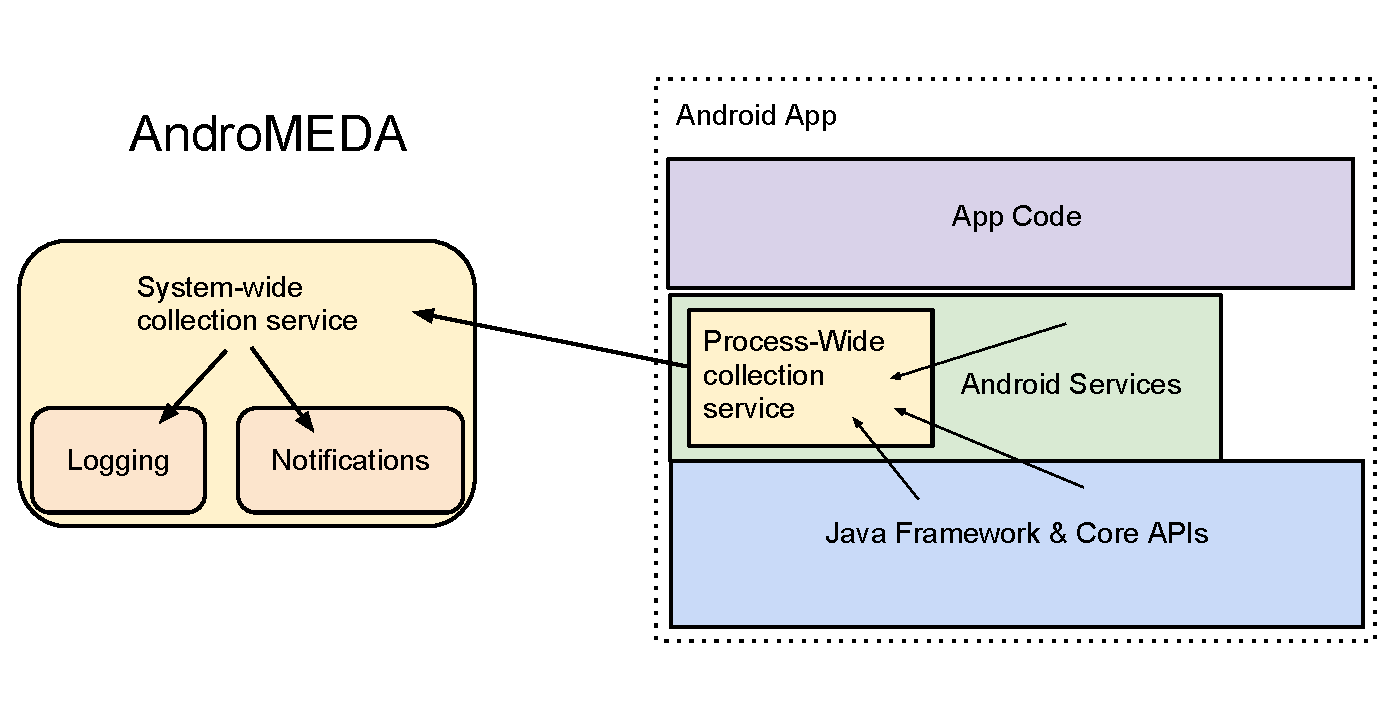
\includegraphics[width=1.0\columnwidth]{figs/AndroMEDA-Architecture-Overview}
\caption{AndroMEDA Architecture Overview}
\label{fig:andromedaoverview}
\end{center}
\end{figure}

The architecture, seen in Figure \ref{fig:andromedaoverview}, is organized into two main parts: A collection of hooks in the API, and a system service to collect this information. The collection of hooks in the API calls into a process-wide service that translates them into events that get sent to the global system service. At the start of every new Dalvik process, the process-wide collector installs hooks into the framework that notifies the collector when the APIs are called.

\begin{figure}[t]
\begin{center}
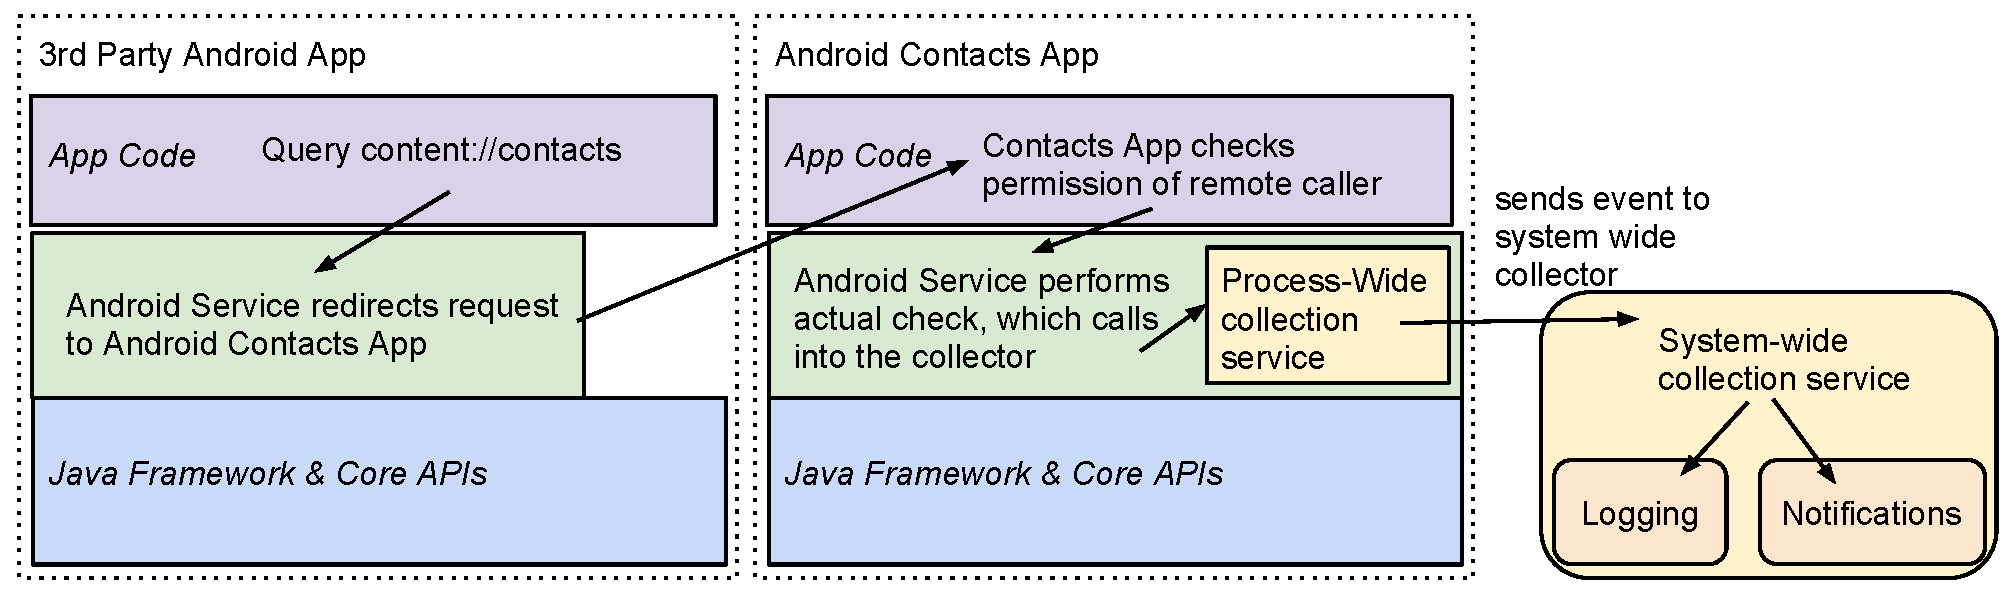
\includegraphics[width=1.0\columnwidth]{figs/AndroMEDA-Inter-App-Example}
\caption{Example code path of an app requesting data from the Contacts app}
\label{fig:interapp-example}
\end{center}
\end{figure}

The hooking mechanisms vary depending on the exact call being instrumented. Android has a standard mechanism for checking permissions in many cases, and we placed a hook where this is enforced. Usually, this takes place during an Remote Procedure Call (RPC) with the process that owns the data - and such, the remote UID is sent along, as seen in Figure \ref{fig:interapp-example}. Unfortunately many permissions are not checked through this manner, but Android Permissions Demystified\citep{felt2011android} has a comprehensive list of API calls and the permissions they require, making it easy to locate essential APIs to instrument. For the more difficult APIs, a static global callback variable is placed in every class we want to instrument. Upon launch of the process, our local collector populates these global variables with callbacks that marshal the data off to the main collection service. Calls are then made to the callback at the appropriate times in the API's normal function, seen in Figure \ref{fig:camera-example}. Using this method, we are able to instrument any API call, getting more data than simply when the permission is checked.

\begin{figure}[t]
\begin{center}
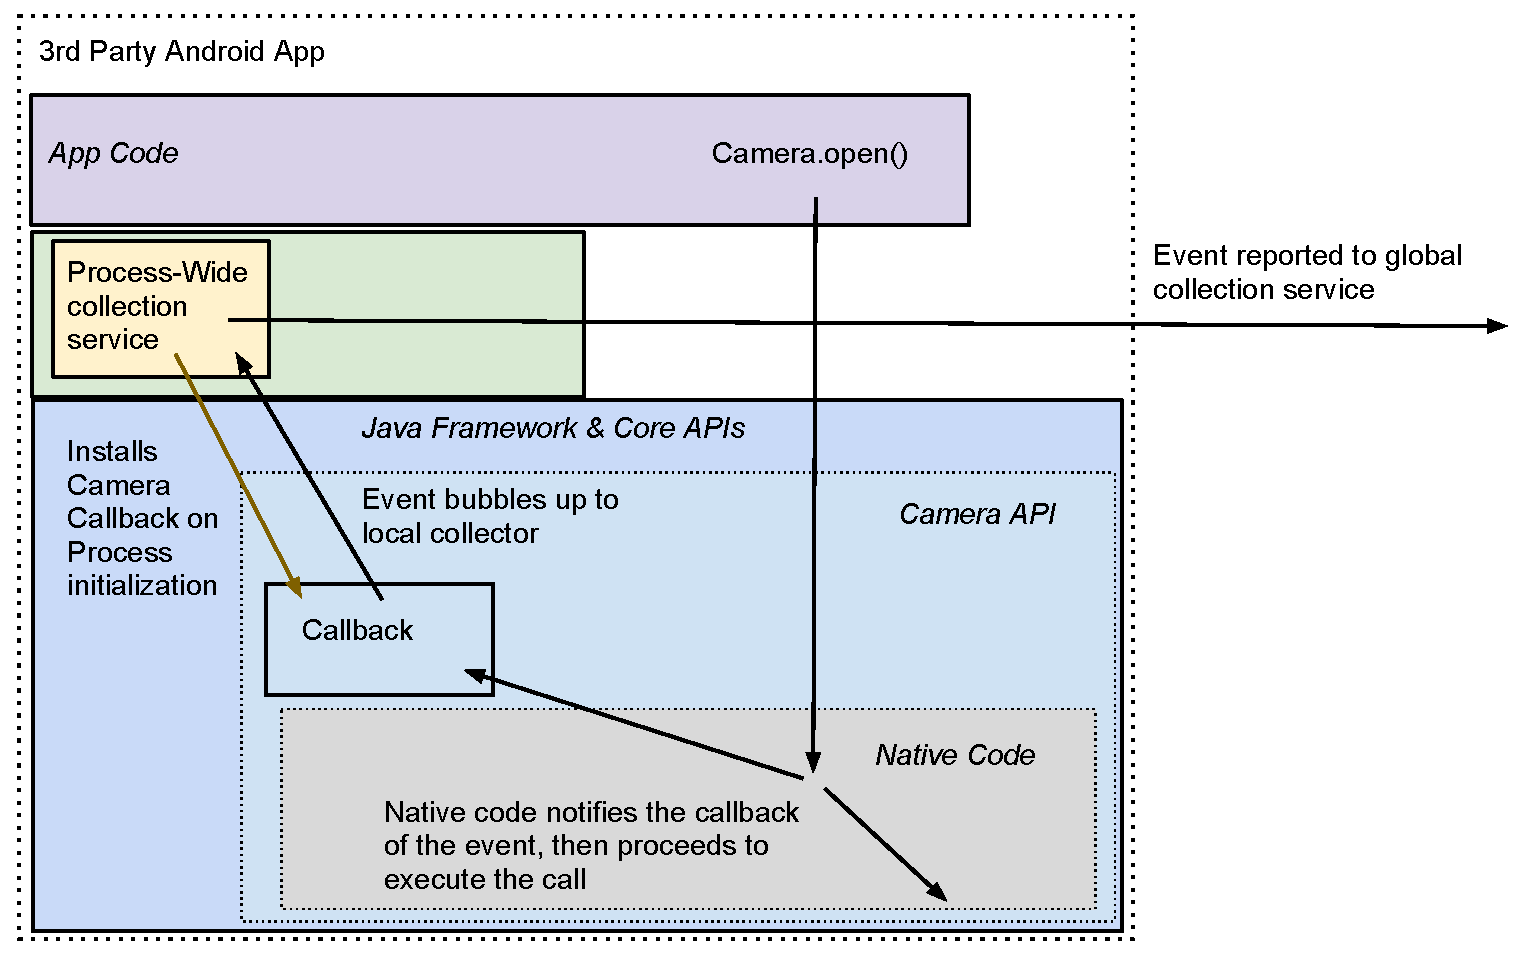
\includegraphics[width=1.0\columnwidth]{figs/AndroMEDA-Static-Example}
\caption{Example code path of instrumenting the Camera API}
\label{fig:camera-example}
\end{center}
\end{figure}

For c and c++ level code, we establish hooks in the Java Native Interface (JNI) - Java's method of communicating with native code - to call back to the main object, since using JNI to call back into Java from c is cumbersome and error prone, which then calls the process-wide callback accordingly, an example can be seen in Figure \ref{fig:camera-example}.

The ability to log virtually any API call is extremely valuable. Not only are permission events logged, but more fine grained events like the starting and stopping of an audio recording can be measured. Internet sockets are logged, along with all POST data set out. Not only is this system light-weight and fast, but it does so with as little modifications as possible. No kernel-level or dalvik-vm-level changes were required.

The global service serves as the central point of collection of all events. It runs in it's own process, and uses Binders (Android's RPC) to communicate with other processes, which feed events into it. These calls are asynchronous, and do not block the remote caller. The service is responsible for logging and processing the events, and taking action on them.

Two way communication is also possible. An app's local collector can query the global service and acquire a list of events for a given package, among other things. This allows user-level apps to be written to leverage AndroMEDAs findings.

\section{Companion App}
A companion app was written, to allow the user to inspect the information being gathered by AndroMEDA. The companion app responds to the Intents broadcast by the notifications that AndroMEDA displays to the user. This brings up a history of events logged by that app, and allows the user to take action. The user may report an app, or uninstall it. A simple web service was set up to aggregate these reports.

The companion app is significant because it does not require the AndroMEDA framework to be present on the phone to function. Despite no local logs being available, the companion app can still query the web service, and view event histories that other users have published.

\chapter{Market Analysis}
\label{sec:market}

In order to evaluate AndroMEDA effectiveness in identifying malware, it's important to evaluate the ability to identify malware without it. As previously discussed in Chapter \ref{sec:permissions}, Permissions are the single security measure that defends an Android user from malicious software. We show a fundamental disconnect between Permissions and UAA, as conclusive evidence that Permissions should not be the sole security system on Android. In order to study this, we must examine the how Permissions reflect app behavior, and if known malware can be identified with Permissions alone.








\section{Android Census}
To do a broad scale study of Android permissions, we introduce a novel dataset: Android Census\citep{androidcensus}. Android Census contains a rich dataset of metadata of apps in the Google Play Store. We first obtain a list of all packages in the Google Play Store from AndroidPit\citep{androidpit}, a 3rd party source that maintains an up-to-date index. We then crawl the GPStore using this list, and insert the data into a MySQL database. See Table \ref{tab:marketstats} for statistics. The metadata described in \ref{tab:marketmetadata} is rich in contextual information about an app. The GPStore was scanned twice per day, generating over 22 million entries, for a period of 1 month in May-June 2012, after which it was stopped\footnote{We plan on continuing scans in the future}. This dataset provides detailed metadata for all apps included in our package list, including the most common apps, but also a larger dataset of lesser known apps (see Figure \ref{tab:downloadstats}). Despite the large amount of metadata available, we will focus on the Permissions, installs, and category, leaving most other fields for Future Work (see Chapter \ref{sec:futurework}).


\begin{table*}[h]
\begin{small}
\begin{tabular}{l|lll}
Scan Timestamp & Number of Apps &  \\
\hline

\textit{fill this in} & I should fill this in  \\

\end{tabular}
\end{small}
%\vspace{-0.2in}
\caption{Statistics from Android Census}
\label{tab:marketstats}
%\vspace{-0.1in}
\end{table*}


\begin{table*}[h]
\begin{small}
\begin{tabular}{r|l}
Metadata & Description \\
\hline

\textit{App Name} & The name of the app, e.g. Google Maps  \\
\textit{App Developer} & The name of the developer, e.g. Google  \\
\textit{Android Version} & The lowest compatible Android version  \\
\textit{Number of Installs} &  The total number of installs. Given as a range. \\
\textit{Description} &  A long (3000 word max) description of the app. \\
\textit{Reviews} &  The user reviews of the app. \\
\textit{Overall Rating} &  The overall rating of the app, from 1 to 5. A user does not need to write a review to leave a rating. \\
\textit{Requested Permissions} &  The list of all the permissions the app requests. \\

\end{tabular}
\end{small}
%\vspace{-0.2in}
\caption{Metadata from Android Census}
\label{tab:marketmetadata}
%\vspace{-0.1in}
\end{table*}


% Should have some figures demonstrating how big this dataset is.

\section{Global Permission Analysis}
We first look at the global trends of Permissions in the GPStore. Ideally, we are in search of a system where access to sensitive PII and dangerous operations is only requested by a handful of apps that truly need them. This would both increases the user's ability to understand how an app behaves, increases the user's trust in the Permission system, and demonstrates a strong connection between Permission Fingerprint and User-App Agreement. Ultimately, however, we find a system that falls short of these goals.

\begin{figure}[h]
\begin{center}
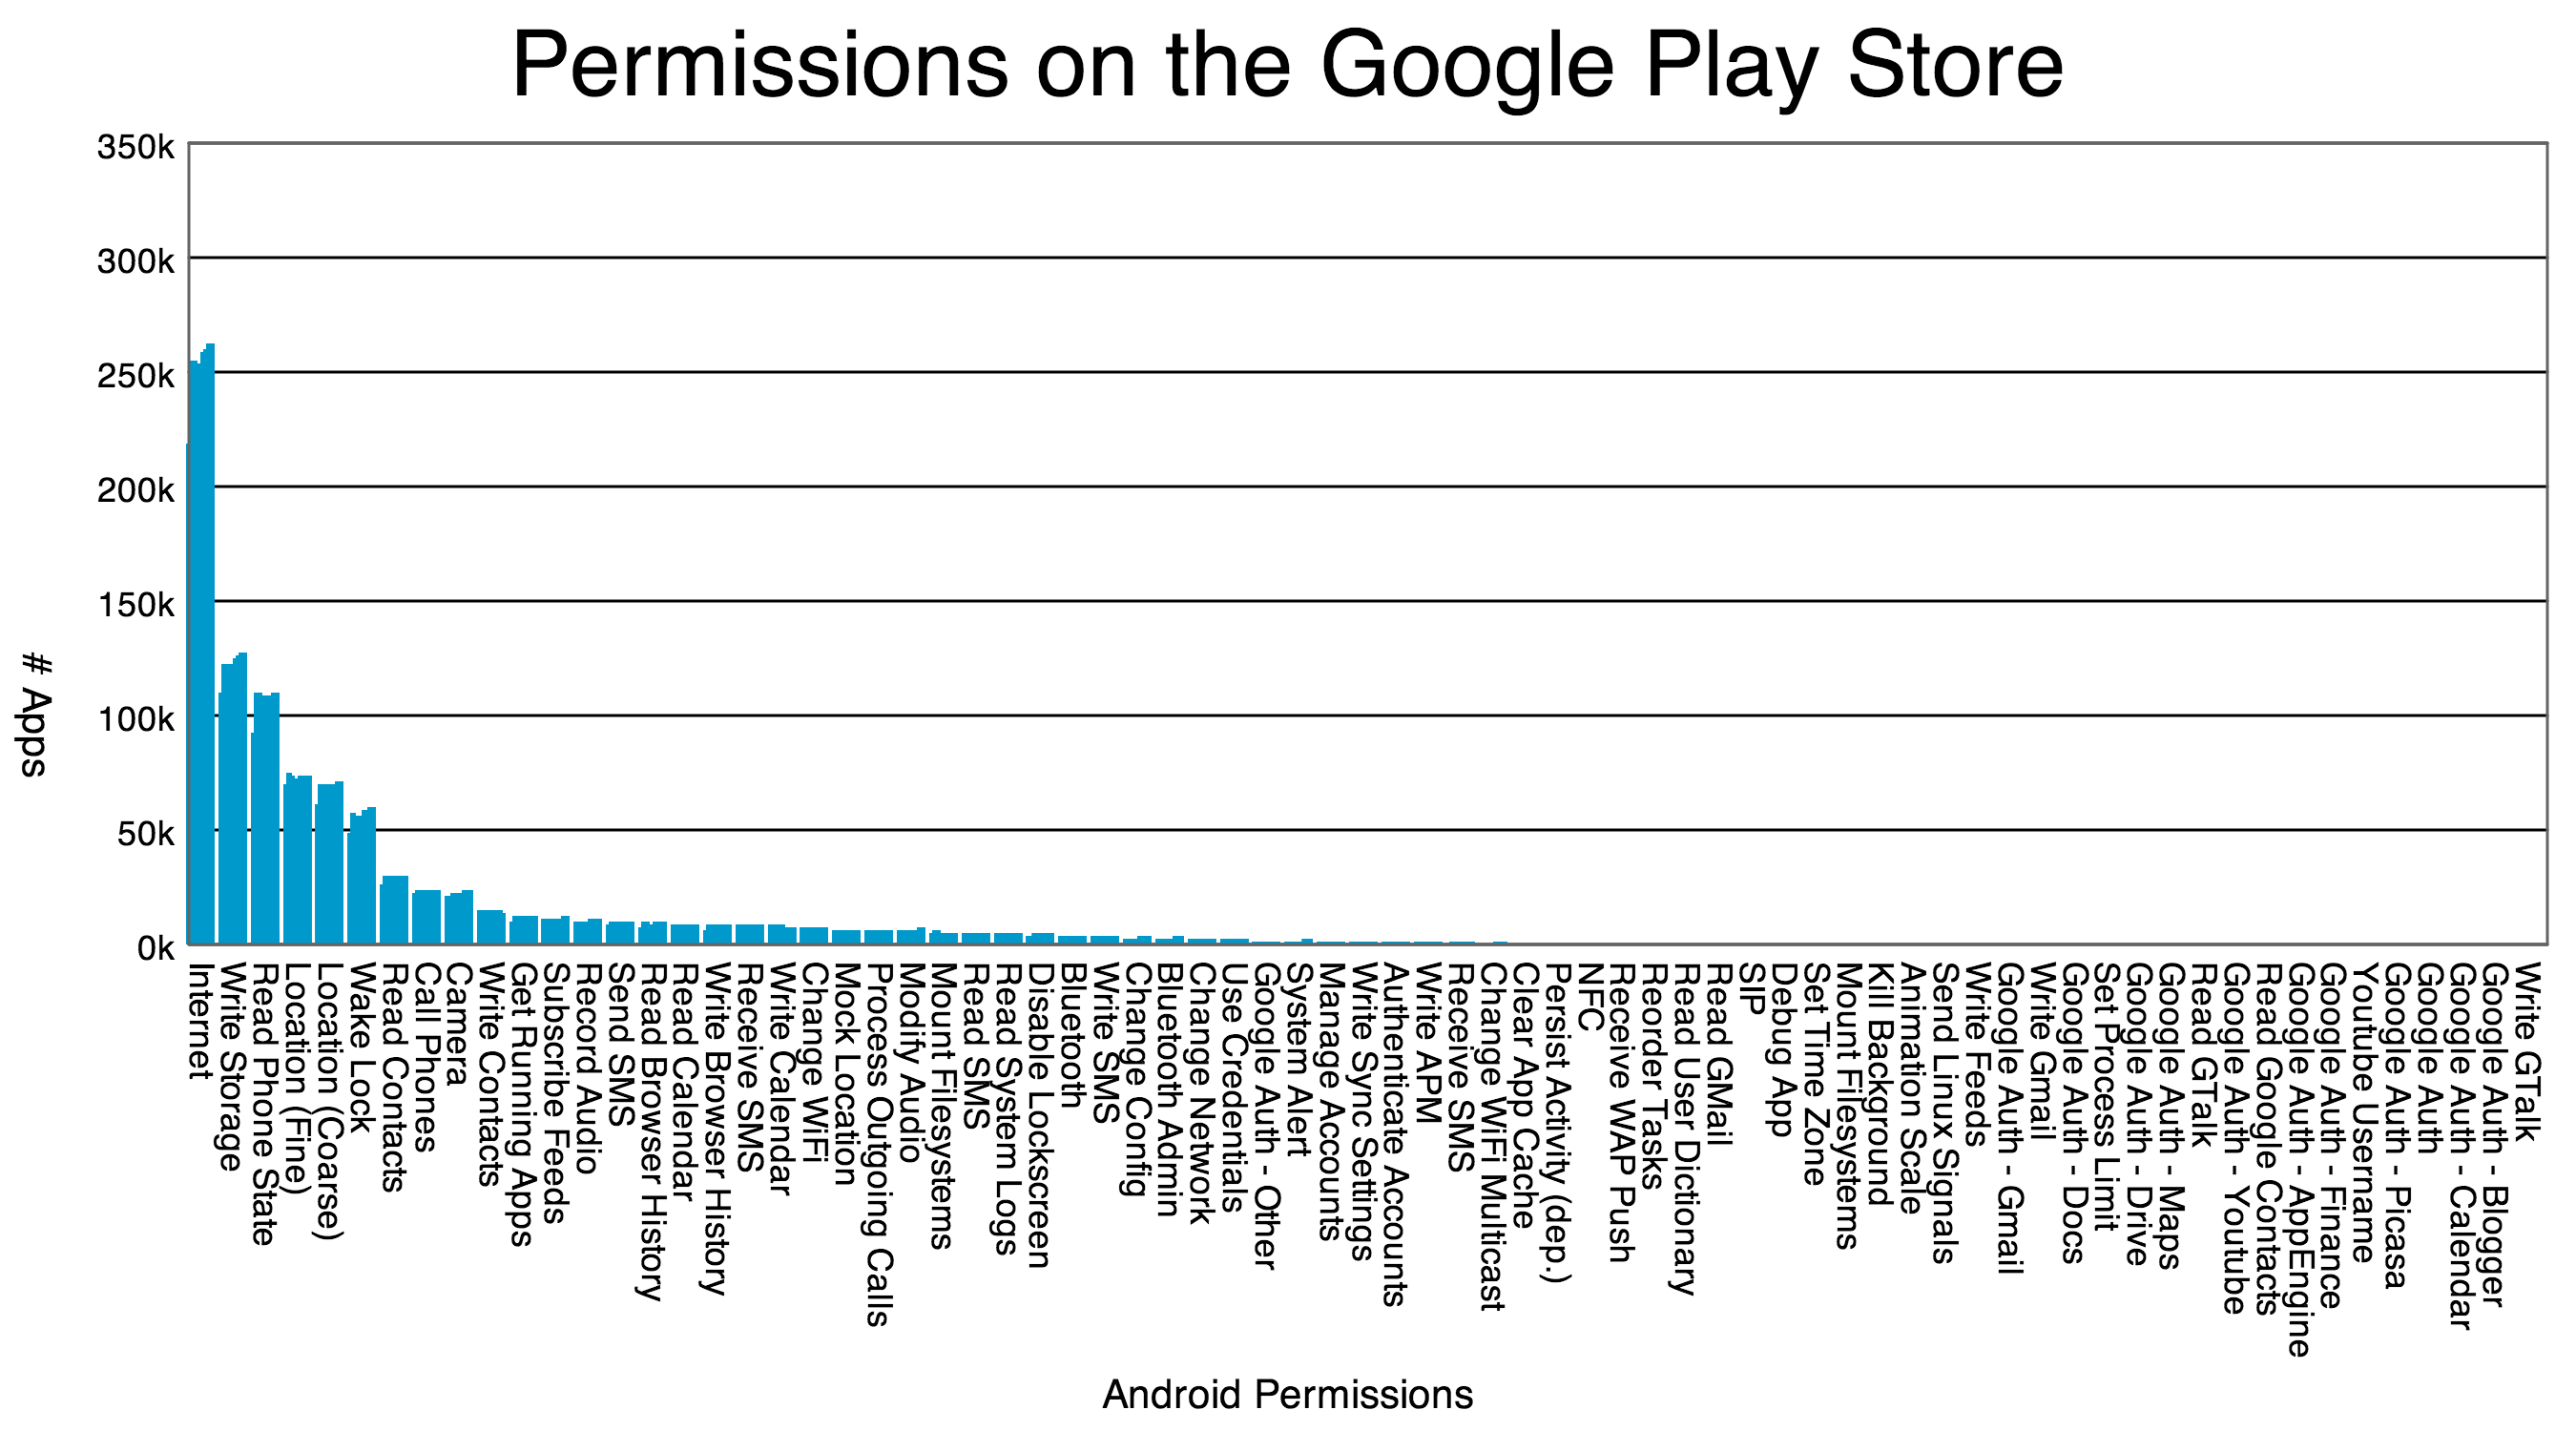
\includegraphics[width=1.0\columnwidth]{figs/AllPermissions}
\caption{Permissions, sorted by how many apps request them in the entire GPStore dataset}
\label{fig:allpermissions}
\end{center}
\end{figure}

\begin{figure}[h]
\begin{center}
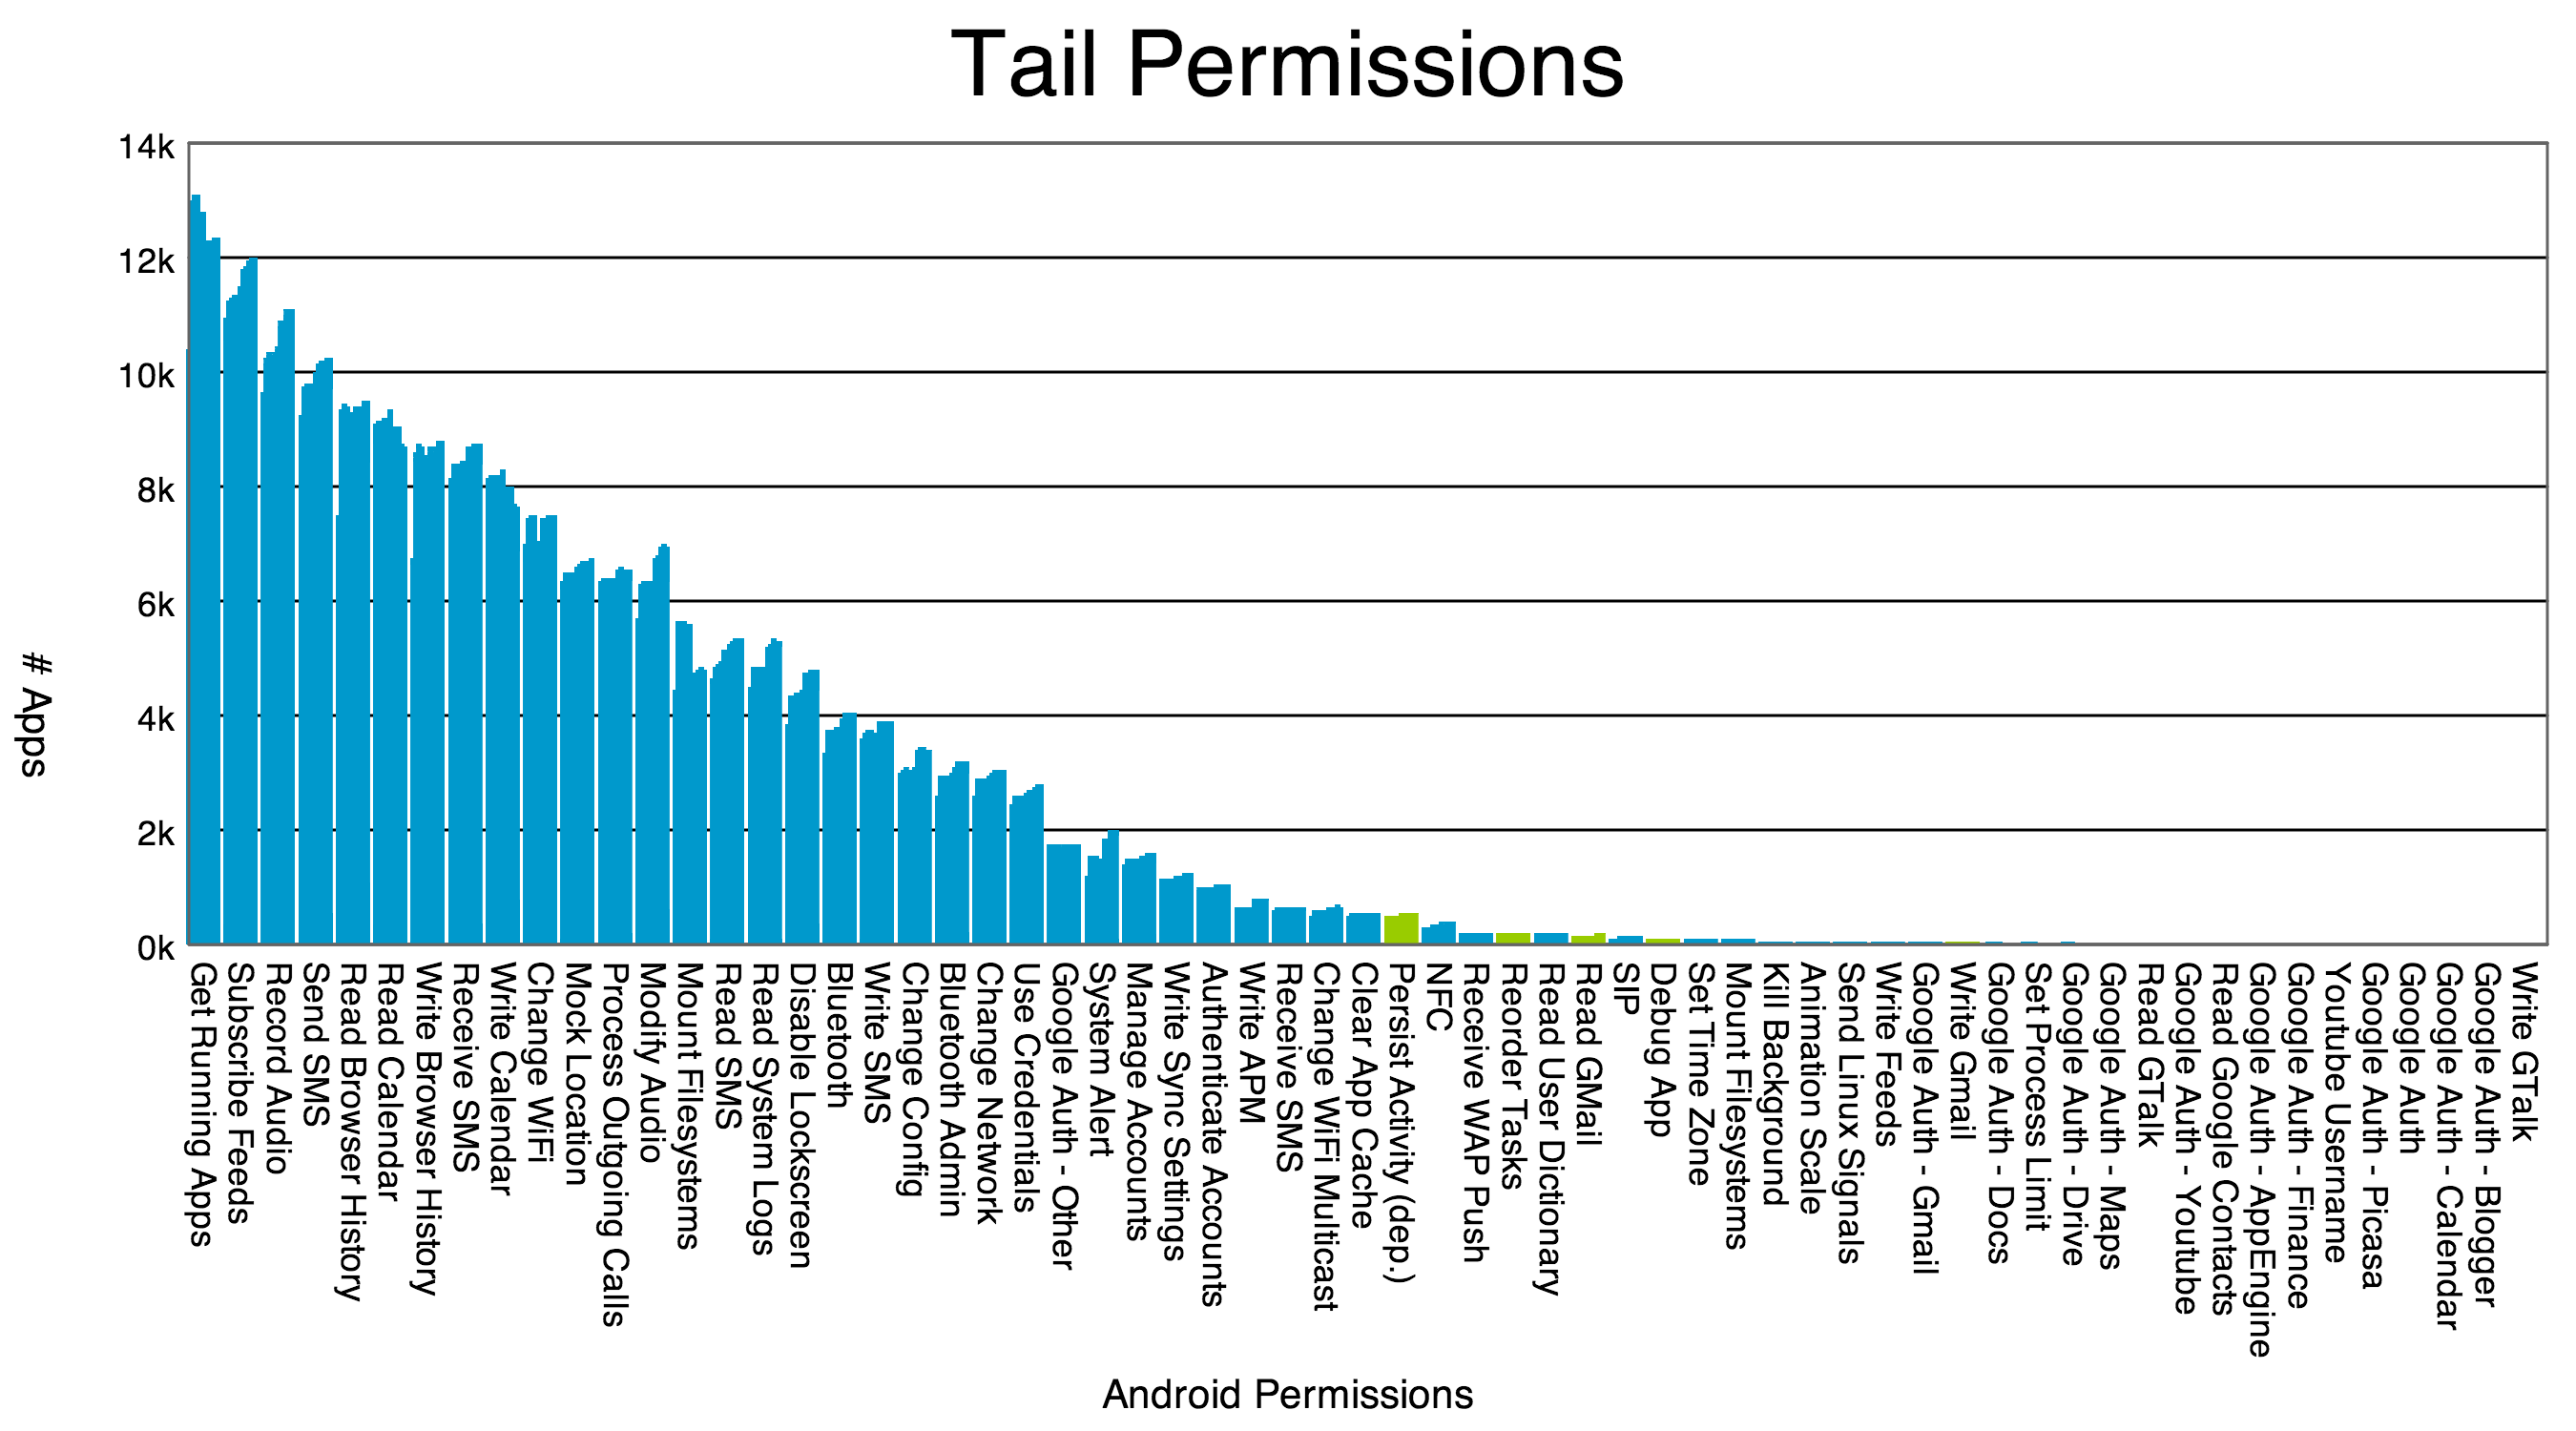
\includegraphics[width=1.0\columnwidth]{figs/AllPermissions_Tail}
\caption{Less commonly used permissions in the GPStore}
\label{fig:tailpermissions}
\end{center}
\end{figure}

Figure \ref{fig:allpermissions} shows all major permissions in the GPStore, sorted by frequency of use. This graph highlights several things: First off, \textit{INTERNET} is a dominant permission, with well over half of the GPStore apps requesting it. The next 5 permissions, \textit{Write to Storage}, \textit{Reading Phone Info}, \textit{Location Info} and \textit{Wake Lock}, all have over 50,000 apps that request them. A steep drop is seen for \textit{Read Contacts}, \textit{Call Phones}, and \textit{Camera}, with around 25,000 apps each. Of these top 9, 3 provide access to semi-personal information: \textit{Reading Phone Info} and the \textit{Location Info} permissions. It's only when we get to the lower 3 do we get access to personal information. 

Figure \ref{fig:tailpermissions} examines the tail permissions in the GPStore. This section contains the bulk of permissions related to PII, with \textit{Record Audio}, \textit{Read Calendar}, \textit{Read SMS}, and so on. It additionally contains many sensitive operations, like \textit{Send SMS} and \textit{System Alert} - which allows apps to draw windows over other apps. These permissions, while being a relatively small portion of the GPStore, still occupy a substantial portion. Indeed, with every dangerous permission, many legitimate use cases can be established that would not violate the UAA, see Figure \ref{tab:permissionsanduses} for examples.

\begin{table*}[h]
\begin{small}
\begin{tabular}{p{3cm}|p{12.5cm}}
Permission & Use Case \\
\hline

\textit{Location (Fine)} & This one has a wide variety of uses, from location-specific news apps and games, to social networks. It's also used by ad networks included in many apps.  \\
\textit{Location (Coarse)} & This one follows the same trends as \textit{Location (Fine)}, but is skewed towards ad networks.  \\
\textit{Read Contacts} & Any access to the address book at all require this, so communication apps, social networks, or many apps that involve sharing with friends will use this.  \\
\textit{Call Phones} & This one is oddly popular. Many customization apps, especially those that seek to replace stock Android apps, will use this, especially if they are replacing address book or home screen functionalities. Additionally, many communication apps will use this, for obvious reasons.  \\
\textit{Camera} & Any photography app or video camera app will make heavy use of this permission. This functionality is often present in other apps as well, e.g. taking a photo of the user for use as a profile photo  \\
\textit{Write Contacts} & This permission is often used with \textit{Read Contacts}. Many social networking sites and services wish to provide ``contact syncing'' abilities with Android device, which requires having write-access to the Contacts database.  \\
\textit{Record Audio} & Like \textit{Camera}, audio apps and communication apps make heavy use of this.  \\
\textit{Send SMS} & Many apps seek to replace the default SMS app, which would therefore require all of the SMS related permissions.  \\
\textit{System Alert} & This permission protects drawing on the screen, on top of other apps. Many apps are designed to be on the screen at all times, either replacing Android components, or complementing them.  \\

\end{tabular}
\end{small}
%\vspace{-0.2in}
\caption{Use cases for common Android Permissions}
\label{tab:permissionsanduses}
%\vspace{-0.1in}
\end{table*}

\subsection{By Market Category}
\label{sec:marketcategory}
Overall, we find many PII related permissions are requested a substantial number of times. A number of use cases exist, but it remains to be seen if the apps follow those use cases. To further examine this, we separate the apps in Android Census into the categories present on the GPStore, and rerun the analysis, seen in Figure \ref{fig:permissionspercategory}.

\begin{figure}[h]
\begin{center}
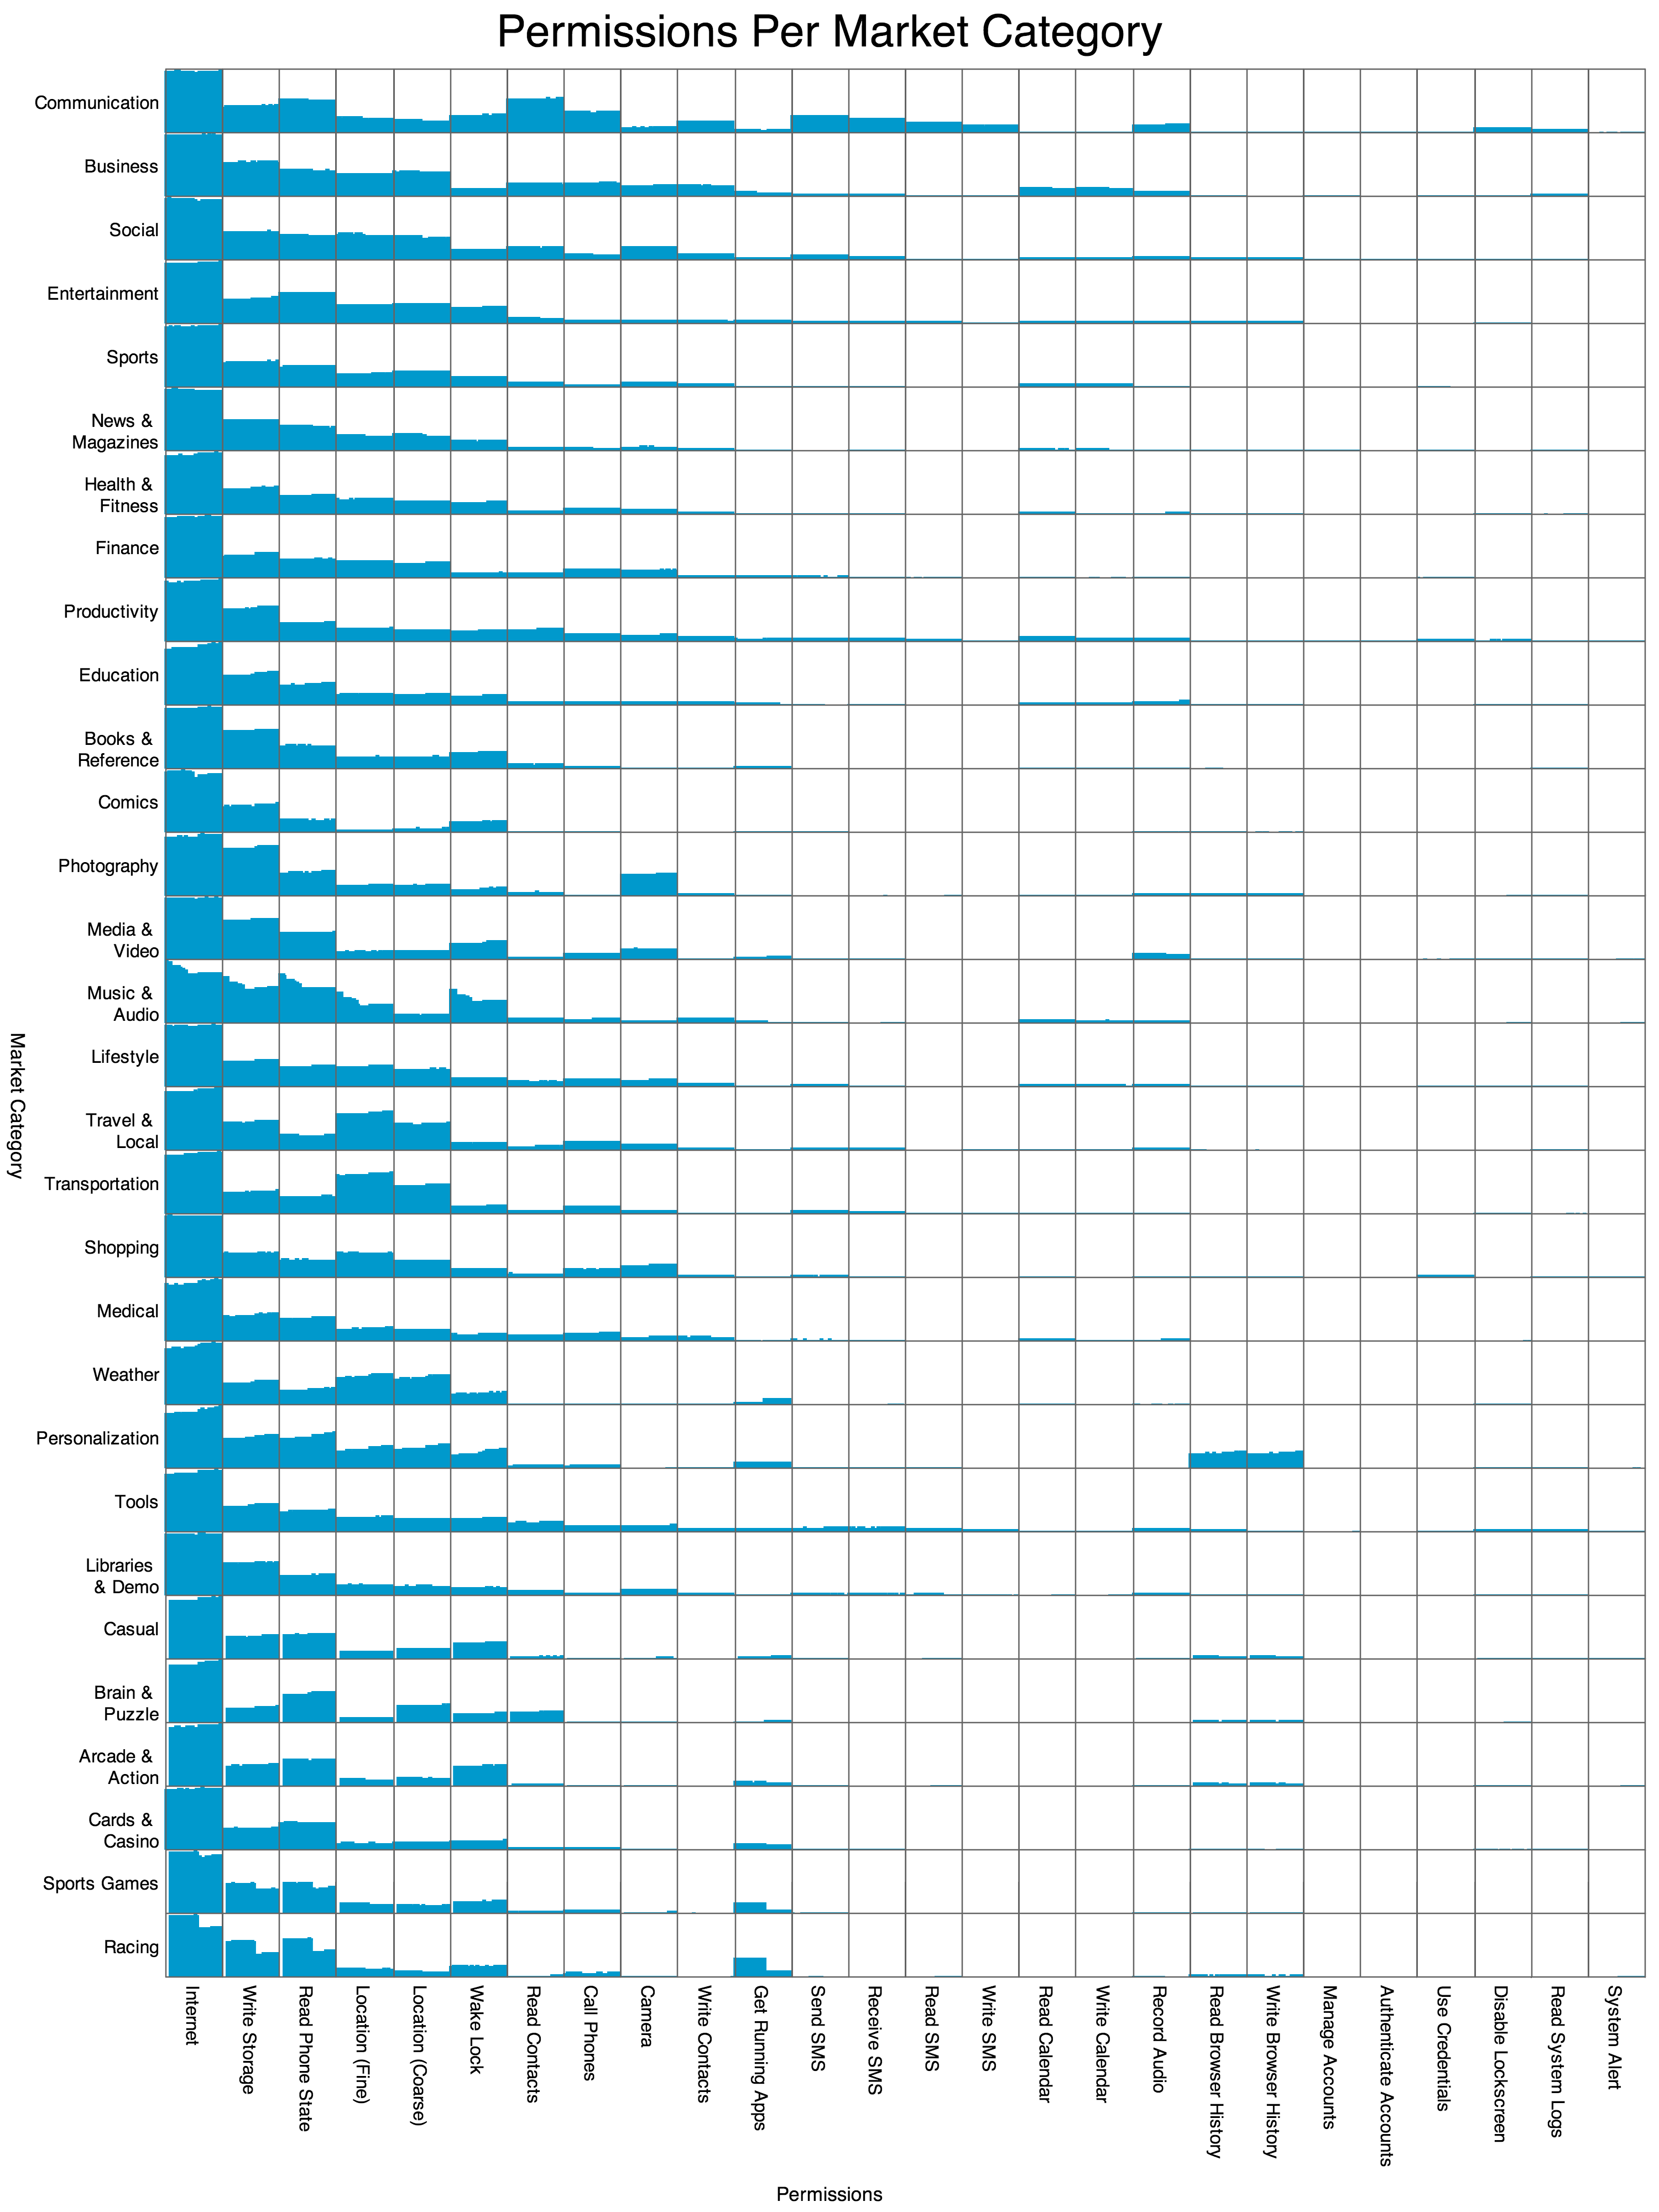
\includegraphics[width=1.0\columnwidth]{figs/PermissionsforMarketCategory}
\caption{Permissions used, as a fraction of total in that category}
\label{fig:permissionspercategory}
\end{center}
\end{figure}

Immediately, the use cases described in \ref{tab:permissionsanduses} become apparent. A large spike is seen in category \textit{Photography} and \textit{Media \& Video} for permission \textit{Camera}, similarly with \textit{Record Audio}, although it's less visible in \textit{Music \& Audio}. Location data is commonly used in \textit{Weather}, \textit{Transportation} and \textit{Travel}, another use case. \textit{Send SMS} is found predominantly in \textit{Communication} and \textit{Social}, another good sign. \textit{Wake Lock} was found heavily in games, music and media, and communication, but less so in other categories, as would be expected for it's use case.

Ultimately, however, some odd patterns can be observed. Despite \textit{Read Contacts} being popular for apps in \textit{Communication}, \textit{Business} and \textit{Social}, it's also found heavily in the \textit{Brain \& Puzzle} game category. A similar pattern is seen in \textit{Call Phones}; it's predominant category is \textit{Communication}, but it's found in significant amounts in \textit{Medical}, \textit{Shopping}, and \textit{Lifestyle}. We also find a spike in \textit{Get Running Apps} in games that does not appear to be present in other market categories. Perhaps the oddest observation was the extremely large spike of \textit{Read Browser History} and \textit{Write Browser History} found in the \textit{Personalization} category.

%\subsubsection{Outliers in \textit{Personalization}}
Isolating the apps in the dataset from category \textit{Personalization} that use the permission \textit{Read Browser History} provides insight into this odd pattern. The most popular app in \textit{Personalization} to use the permission is an app called Launcher Pro\citep{launcherpro}. Downloaded over 10 Million times, with an average rating of 4.5, LauncherPro is a highly respected 3rd party Android Home Screen. It has 181,628 5 star ratings, and only 8,230 1 star reviews. The permission comes from a set of widgets to access the browser shortcuts from the home screen.

The next most popular apps in \textit{Personalization} that use permission \textit{Read Browser History} are Seabed Live Wallpaper\citep{seabedlivewallpaper} and Heart Live Wallpaper\citep{heartlivewallpaper}, both by the same developer ``Good LiveWallpaper''\citep{goodlivewallpaper}. These two apps have each been downloaded over 1 Million times, and have an average rating of 3.8 and 4.1, respectively. However, the bad reviews for both apps make numerous references to poor behavior, with one user saying ``The sheer number of push ads this single dud of a wallpaper shoves on your phone is astounding.''\citep{seabedlivewallpaper}. It's clear these apps does not use \textit{Read Browser History} for a trusted purpose, but rather for advertising.

Despite the fact that the two apps come from the same market category, and use the same permissions, they have vastly different expected behavior and UAA, one of which violates it frequently, and the other is highly trusted. Permissions, while being used rather judiciously in many parts of the market, clearly have times when they are requested without truely needing them. These situations degrade the effectiveness of permissions, because the user lacks a trustworthy reason why the app requires such capabilities.

%Overall, we've noted a number of times when patterns in permissions in the GPStore break our expectations of them - potentially violating them User-App Agreement. These could be detected simply from the Permission Fingerprint. We have shown a fairly strong correlation with major PII permissions and Android categories, but demonstrated many cases where they do not line up, both maliciously and with legitimate use cases.






\section{Android Malware Genome Project}
Next, we project a malware dataset onto the Android Census, with the goal of idenitifying their Permission Fingerprints as potential outliers. Ideally, all malicious behavior would show up in the permission fingerprint of an app, so therefore it's unique set of capabilities would stand out in the Google Play Store, thus showing a strong correlation between expected behavior and Permission Fingerprint. Upon further exploration, we find many patterns of malware are easily identifiable through the Permission Fingerprint, but some behavior passes by unnoticed, demonstrating the need for AndroMEDA.

The dataset we use - the largest academic set of it's kind, is the Android Malware Genome Project\citep{zhou2012dissecting}, from NCSU. Containing almost 1300 samples from 52 families of actual Android malware, it provides the ideal test dataset for Android. 

\begin{figure}[h]
\begin{center}
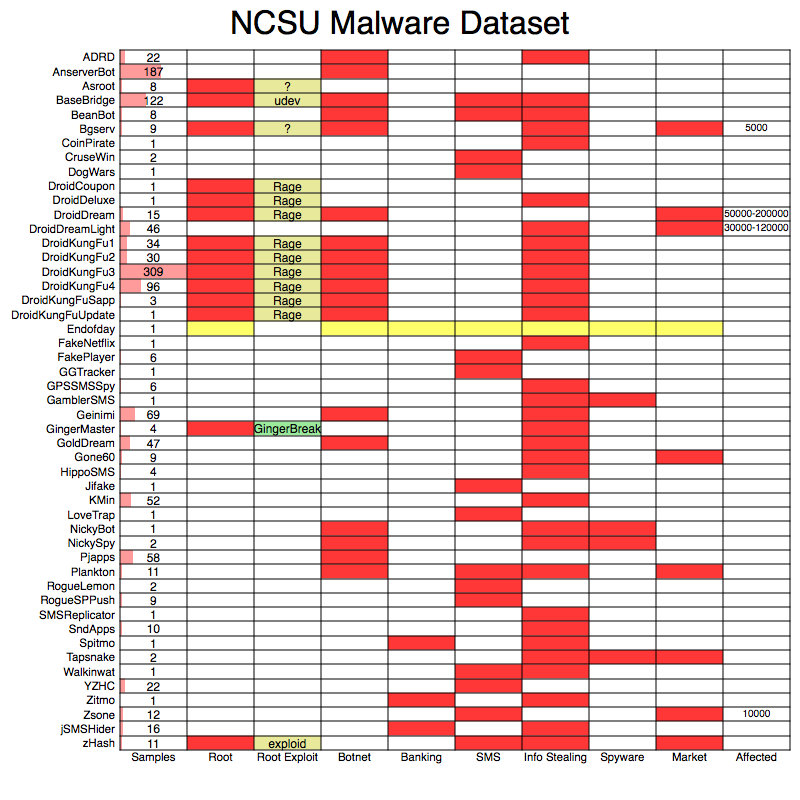
\includegraphics[width=0.85\columnwidth]{figs/NCSUMalwareDataset}
\caption{A summary of the malware families found in the Android Malware Genome Project, see Figure \ref{tab:malwaredbcategories} for explanations of the classes}
\label{fig:malwaredboverview}
\end{center}
\end{figure}

\begin{table*}[h]
\begin{small}
\begin{tabular}{p{3cm}|p{12.5cm}}
Malware Class & Description \\
\hline

\textit{Root} & The malware uses a rootkit as a method of attack.    \\
\textit{Botnet} & The malware exhibits behavior associated with botnets, e.g. accepts remote commands.    \\
\textit{Banking} & The malware is designed specifically to intercept Banking messages.    \\
\textit{SMS} & The malware sends Premium SMS messages charged against the user.    \\
\textit{Info} &  The malware uploads personal information to a remote server, without notifying the user   \\
\textit{Spyware} & The malware remains on in the background, or has the capability of remotely monitoring the smartphone user.    \\
\textit{Market} &  The malware was spotted in the official Google Play Store   \\

\end{tabular}
\end{small}
%\vspace{-0.2in}
\caption{Malware Classes found in the Android Malware Genome Project}
\label{tab:malwaredbcategories}
%\vspace{-0.1in}
\end{table*}


\subsection{Classification}
We first classify each malware family by its capabilities, according to data aggregated by Spreitzenbarth\citep{spreitzenbarth2013} and Hackmageddon\citep{hackmageddon2011}, with the chart shown in Figure \ref{fig:malwaredboverview}, and the explanation of the classification of capabilities in Table \ref{tab:malwaredbcategories}.

Of the three classes of malware discussed in Chapter \ref{sec:malware}, we observe that very few of the malware families use only one attack vector - 6 families, all of which only used \textit{SMS} attacks, and 1, \textit{Pjapps} used none, only being a botnet. Clearly, Android Malware often uses multiple vectors. We also note that 33 of 52 - 63\% of all malware families upload personal information to a remote server. 

\begin{figure}[h]
\begin{center}
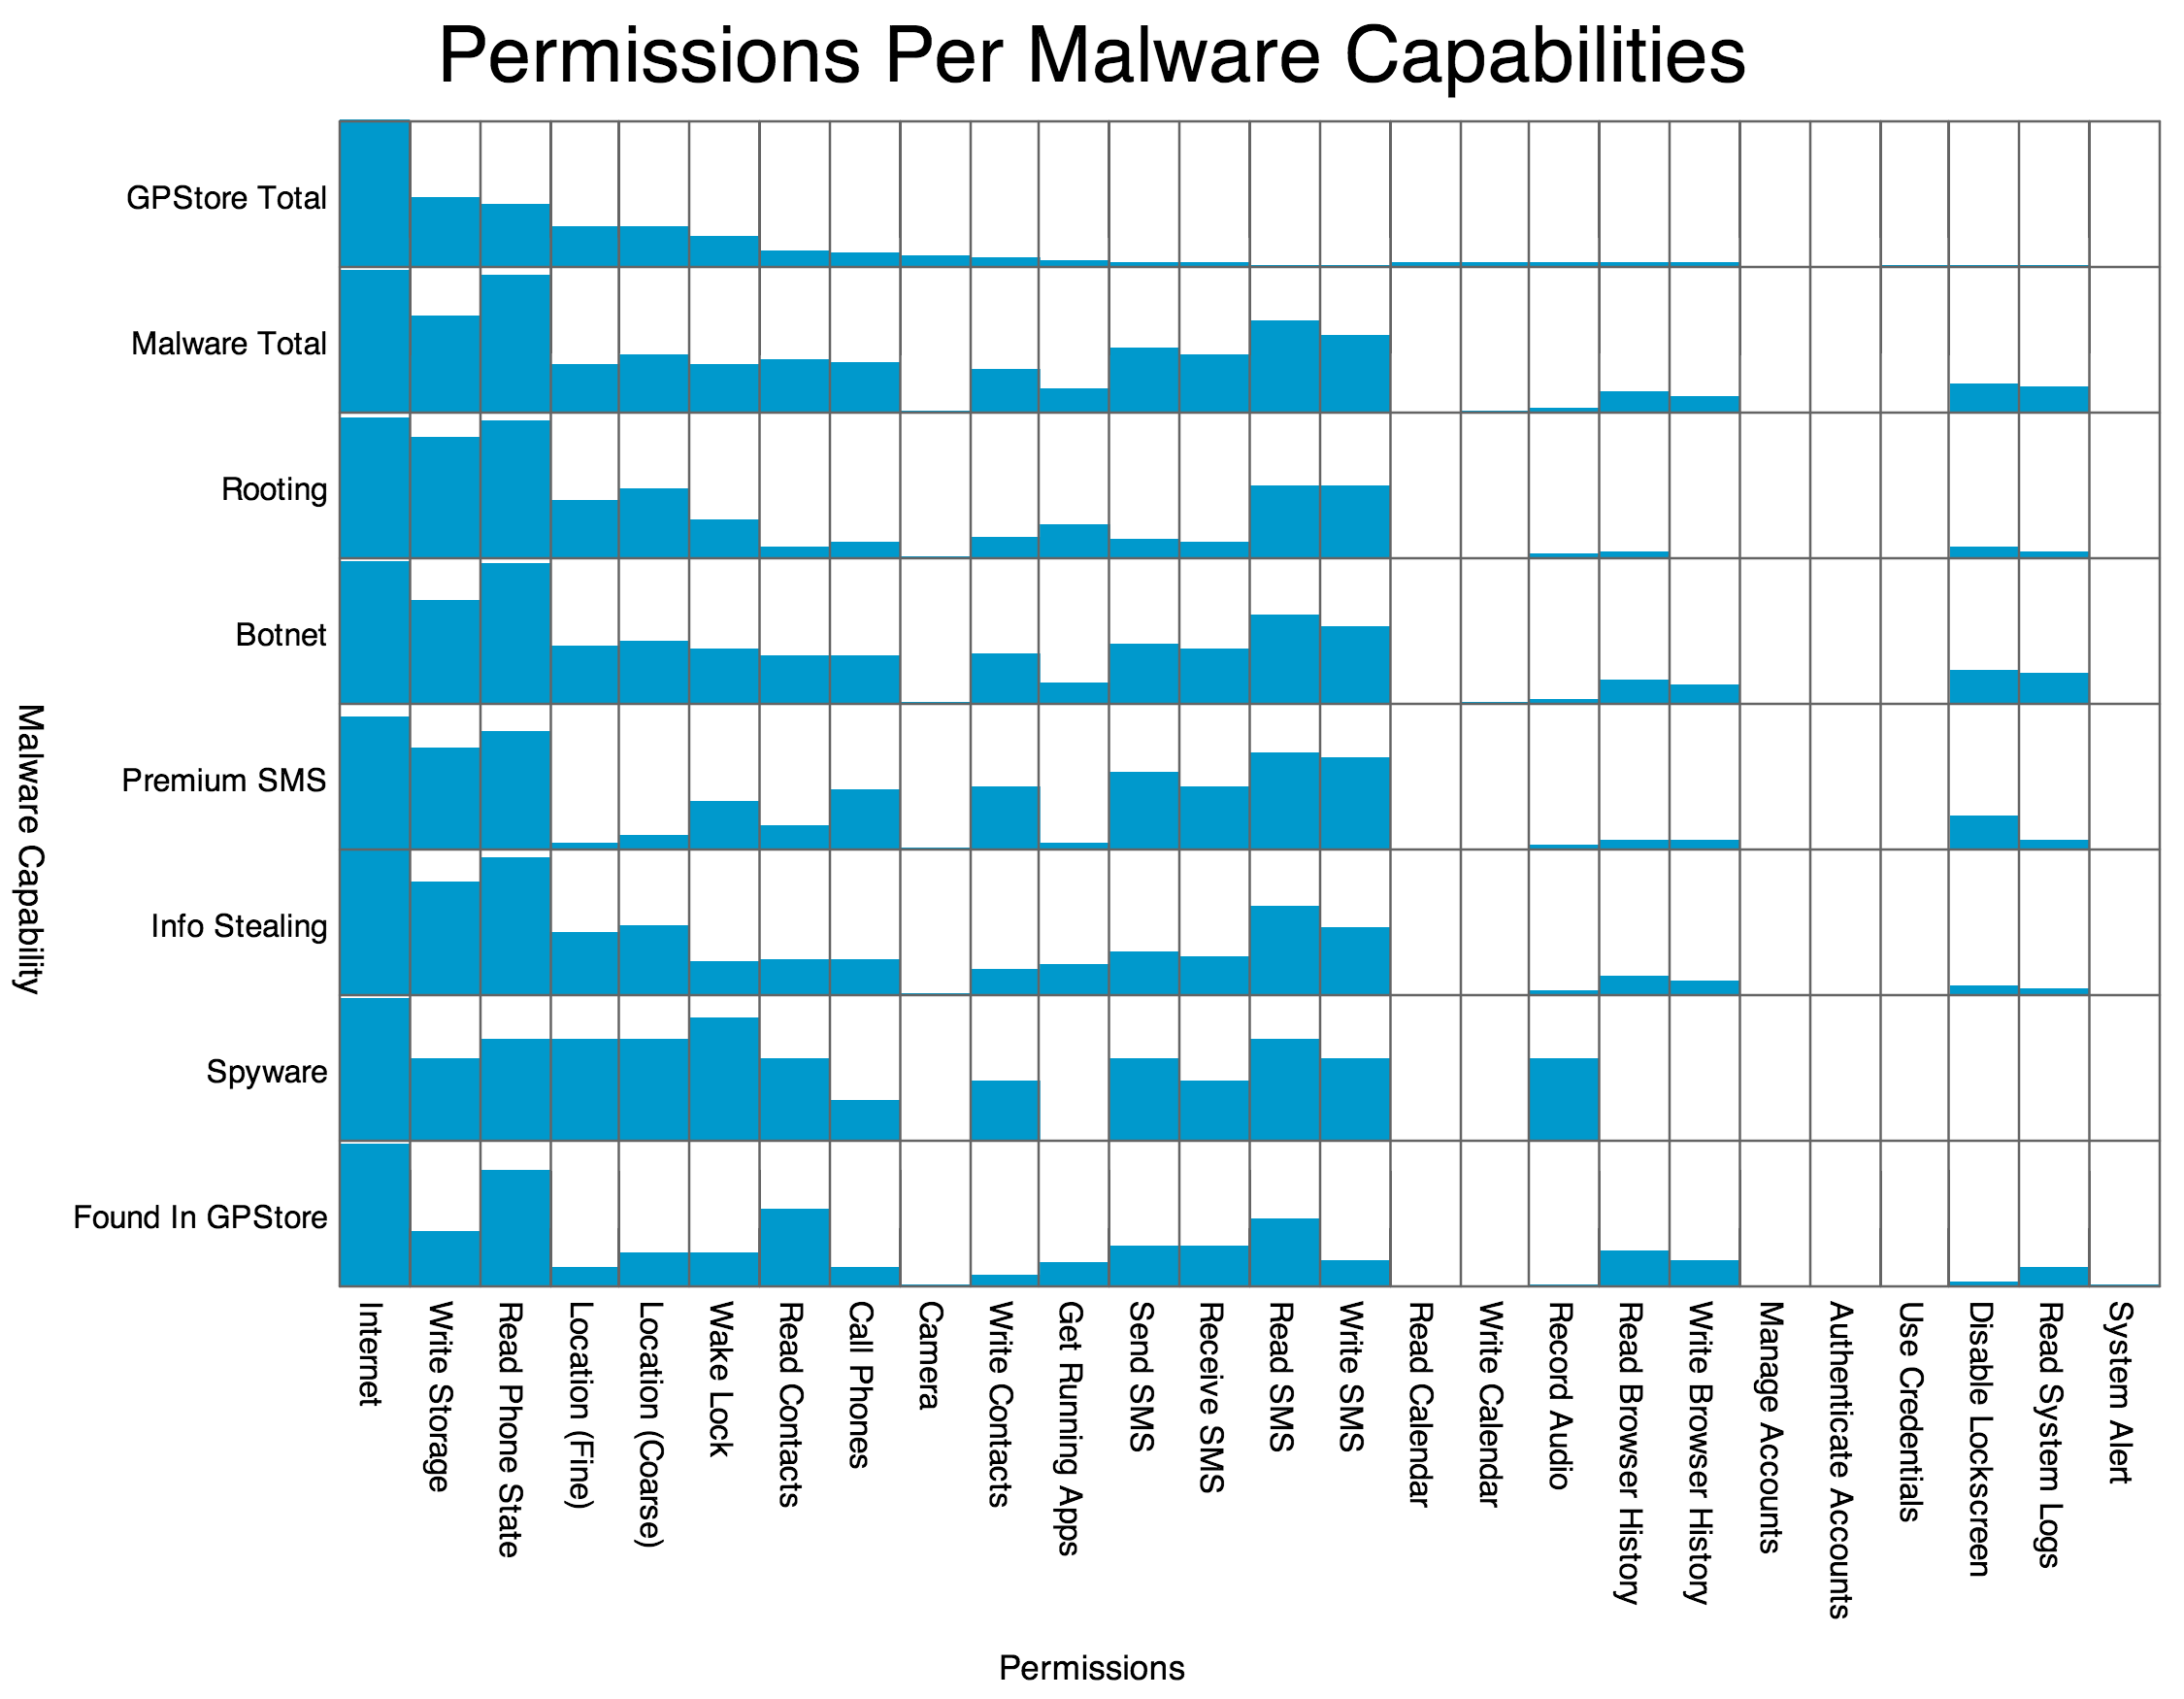
\includegraphics[width=1.0\columnwidth]{figs/MalwareCapabiltiesPermissions}
\caption{Permission Fingerprints of malware with different capabilties, compared to the GPStore total}
\label{fig:malwarefingerprint}
\end{center}
\end{figure}

\subsection{Fingerprints}
The first step in analyzing whether malware Permission Fingerprints are seen as outliers is to obtain permission fingerprints for all apps in the database. After which, we aggregated the fingerprints by classification of capabilities. The result, Figure \ref{fig:malwarefingerprint}, provides a novel look at malware, it's capabilities, and it's permissions relative to the Android market. The differences in Permission Fingerprints, and therefore capabilities of Malware vs the GPStore total become obvious right away. Malware is far more likely to request access to SMS, particularly reading and writing the database, as well as system operations like disabling the lock screen and reading system logs. 

However, further insight is given when looking at the fingerprints of malware with a specific capability. \textit{Spyware} apps demonstrate this quite clearly: They request access to location, permission to keep the device on at all times, record audio and send SMS messages. These capabilities are what would be expected out of spyware. Likewise, \textit{Premium SMS} apps requested access to Send SMS messages quite often\footnote{The reason this number is not 100\% is because not all variants of a family of malware known to posses a \textit{Premium SMS} exploit may have that capability}. We also observe that \textit{Botnet} malware occasionally accesses system features like disabling the lock screen and reading system logs.

These obversvations are highly valuble, but things break down when we look at the \textit{Info} category. This permission fingerprint, aside from \textit{Read SMS} and \textit{Write SMS}, does not appear significantly different than the GPStore total, especially when considering the Market Category fluctuations observed earlier in Section \ref{sec:marketcategory}. 


\section{By Install Count}
As we have shown, all categories of malware but Info Theft Malware show profound differences in permission fingerprints: they are far more likely to access unusual permissions than normal Android apps. However, Info Theft apps did not show such anomalies, making them far easier to hide inside of benign apps - a technique malware writers already use\citep{avastfakeapps}. Thus, if more popular apps have more access to PII, this vector poses a serious threat.

For starters, we note that the metadata in Android Census doesn't give precise download measurements, but rather broad ranges, as seen in Figure \ref{fig:gpstoreapps}. We plot these in Table \ref{tab:downloadstats}, noting the number of apps in each download range, and it's total percent of all downloads in the market. The top percentile, only 9 apps, accounts for an estimated\footnote{The formula for estimated total downloads was taking the average of the download range, and multiplying it by the number of apps} 11\% of all downloads, and apps over 1 million downloads - only 2250 apps in total - account for an estimated 70\% of all downloads in the entire Google Play Store.

\begin{table*}[h]
\begin{small}
\begin{tabular}{r|llll}
Download Range & Number of Apps & Estimated Total Downloads & Percent of All Downloads & Aggregate Percentage \\
\hline

\textit{100M-500M} & 9 & 2.7B & 11.78\% & 11.78\% \\
\textit{50M-100M} & 12 & 900.0M & 3.93\% & 15.71\% \\
\textit{10M-50M} & 165 & 4.95B & 21.6\% & 37.31\% \\
\textit{5M-10M} & 279 & 2.09B & 9.13\% & 46.44\% \\
\textit{1M-5M} & 1785 & 5.36B & 23.36\% & 69.8\% \\
\textit{500K-1M} & 2010 & 1.51B & 6.58\% & 76.38\% \\
\textit{100K-500K} & 10483 & 3.14B & 13.72\% & 90.1\% \\
\textit{50K-100K} & 9363 & 702.23M & 3.06\% & 93.16\% \\
\textit{10K-50K} & 37925 & 1.14B & 4.96\% & 98.13\% \\
\textit{5K-10K} & 24872 & 186.54M & 0.81\% & 98.94\% \\
\textit{1K-5K} & 66587 & 199.76M & 0.87\% & 99.81\% \\
\textit{500-1K} & 28676 & 21.51M & 0.09\% & 99.91\% \\
\textit{100-500} & 59616 & 17.88M & 0.08\% & 99.98\% \\
\textit{50-100} & 23394 & 1.75M & 0.01\% & 99.99\% \\
\textit{10-50} & 53343 & 1.6M & 0.01\% & 100.0\% \\
\textit{5-10} & 13720 & 96.04K & 0.0\% & 100.0\% \\
\textit{1-5} & 30541 & 91.62K & 0.0\% & 100.0\% \\
\textit{0-0} & 7694 & 0.0 & 0.0\% & 100.0\% \\

\end{tabular}
\end{small}
%\vspace{-0.2in}
\caption{App download statistics from Android Census}
\label{tab:downloadstats}
%\vspace{-0.1in}
\end{table*}

%\subsection{Top 9 Apps}
%The top 9 apps (in no particular order), are \textit{Facebook}, \textit{GMail}, \textit{Google Maps}, \textit{Google Street View}, \textit{Google Search}, \textit{Google Voice Search}, \textit{Youtube} and \textit{Adobe Flash Player}. It's intriguing yet understandable to see so many Google apps in the top spots, but this is understandable given the fact that these apps have been in the market since very early on.

%The permissions these apps request is atypical of most apps in the GPStore. \textit{Adobe Flash Player} requests no permissions at all, but this is due to it's role as a browser plugin, and is an outlier in this. 

%\subsection{Apps over 1 Million Downloads}
%\temp{Show the same permission histogram as before, but each row is a different download range}

%Discuss it.
Figure \ref{fig:topappsfingerprint} shows the permission fingerprints of the top download categories on the Google Play Store. The apps in the lower ranges, from 10K-50K, show a fingerprint very similar to the overall plot. However, as the install counts rise, several very key permissions rise as well. \textit{Get Running Apps}, \textit{Camera}, \textit{Record Audio}, \textit{Read Contacts}, and \textit{Wake Lock} all spike in popularity, the more installs the app has. These permissions are especially sensitive PII related permissions. Towards the very top, even more permissions become used, \textit{Read and Write SMS} and \textit{Read Browser History}, which are also extremely common malware permissions. Overall, aside from \textit{Read and Write SMS}, the \textit{Info Theft} malware described above has a surprisingly similar permission fingerprint.

\begin{figure}[h]
\begin{center}
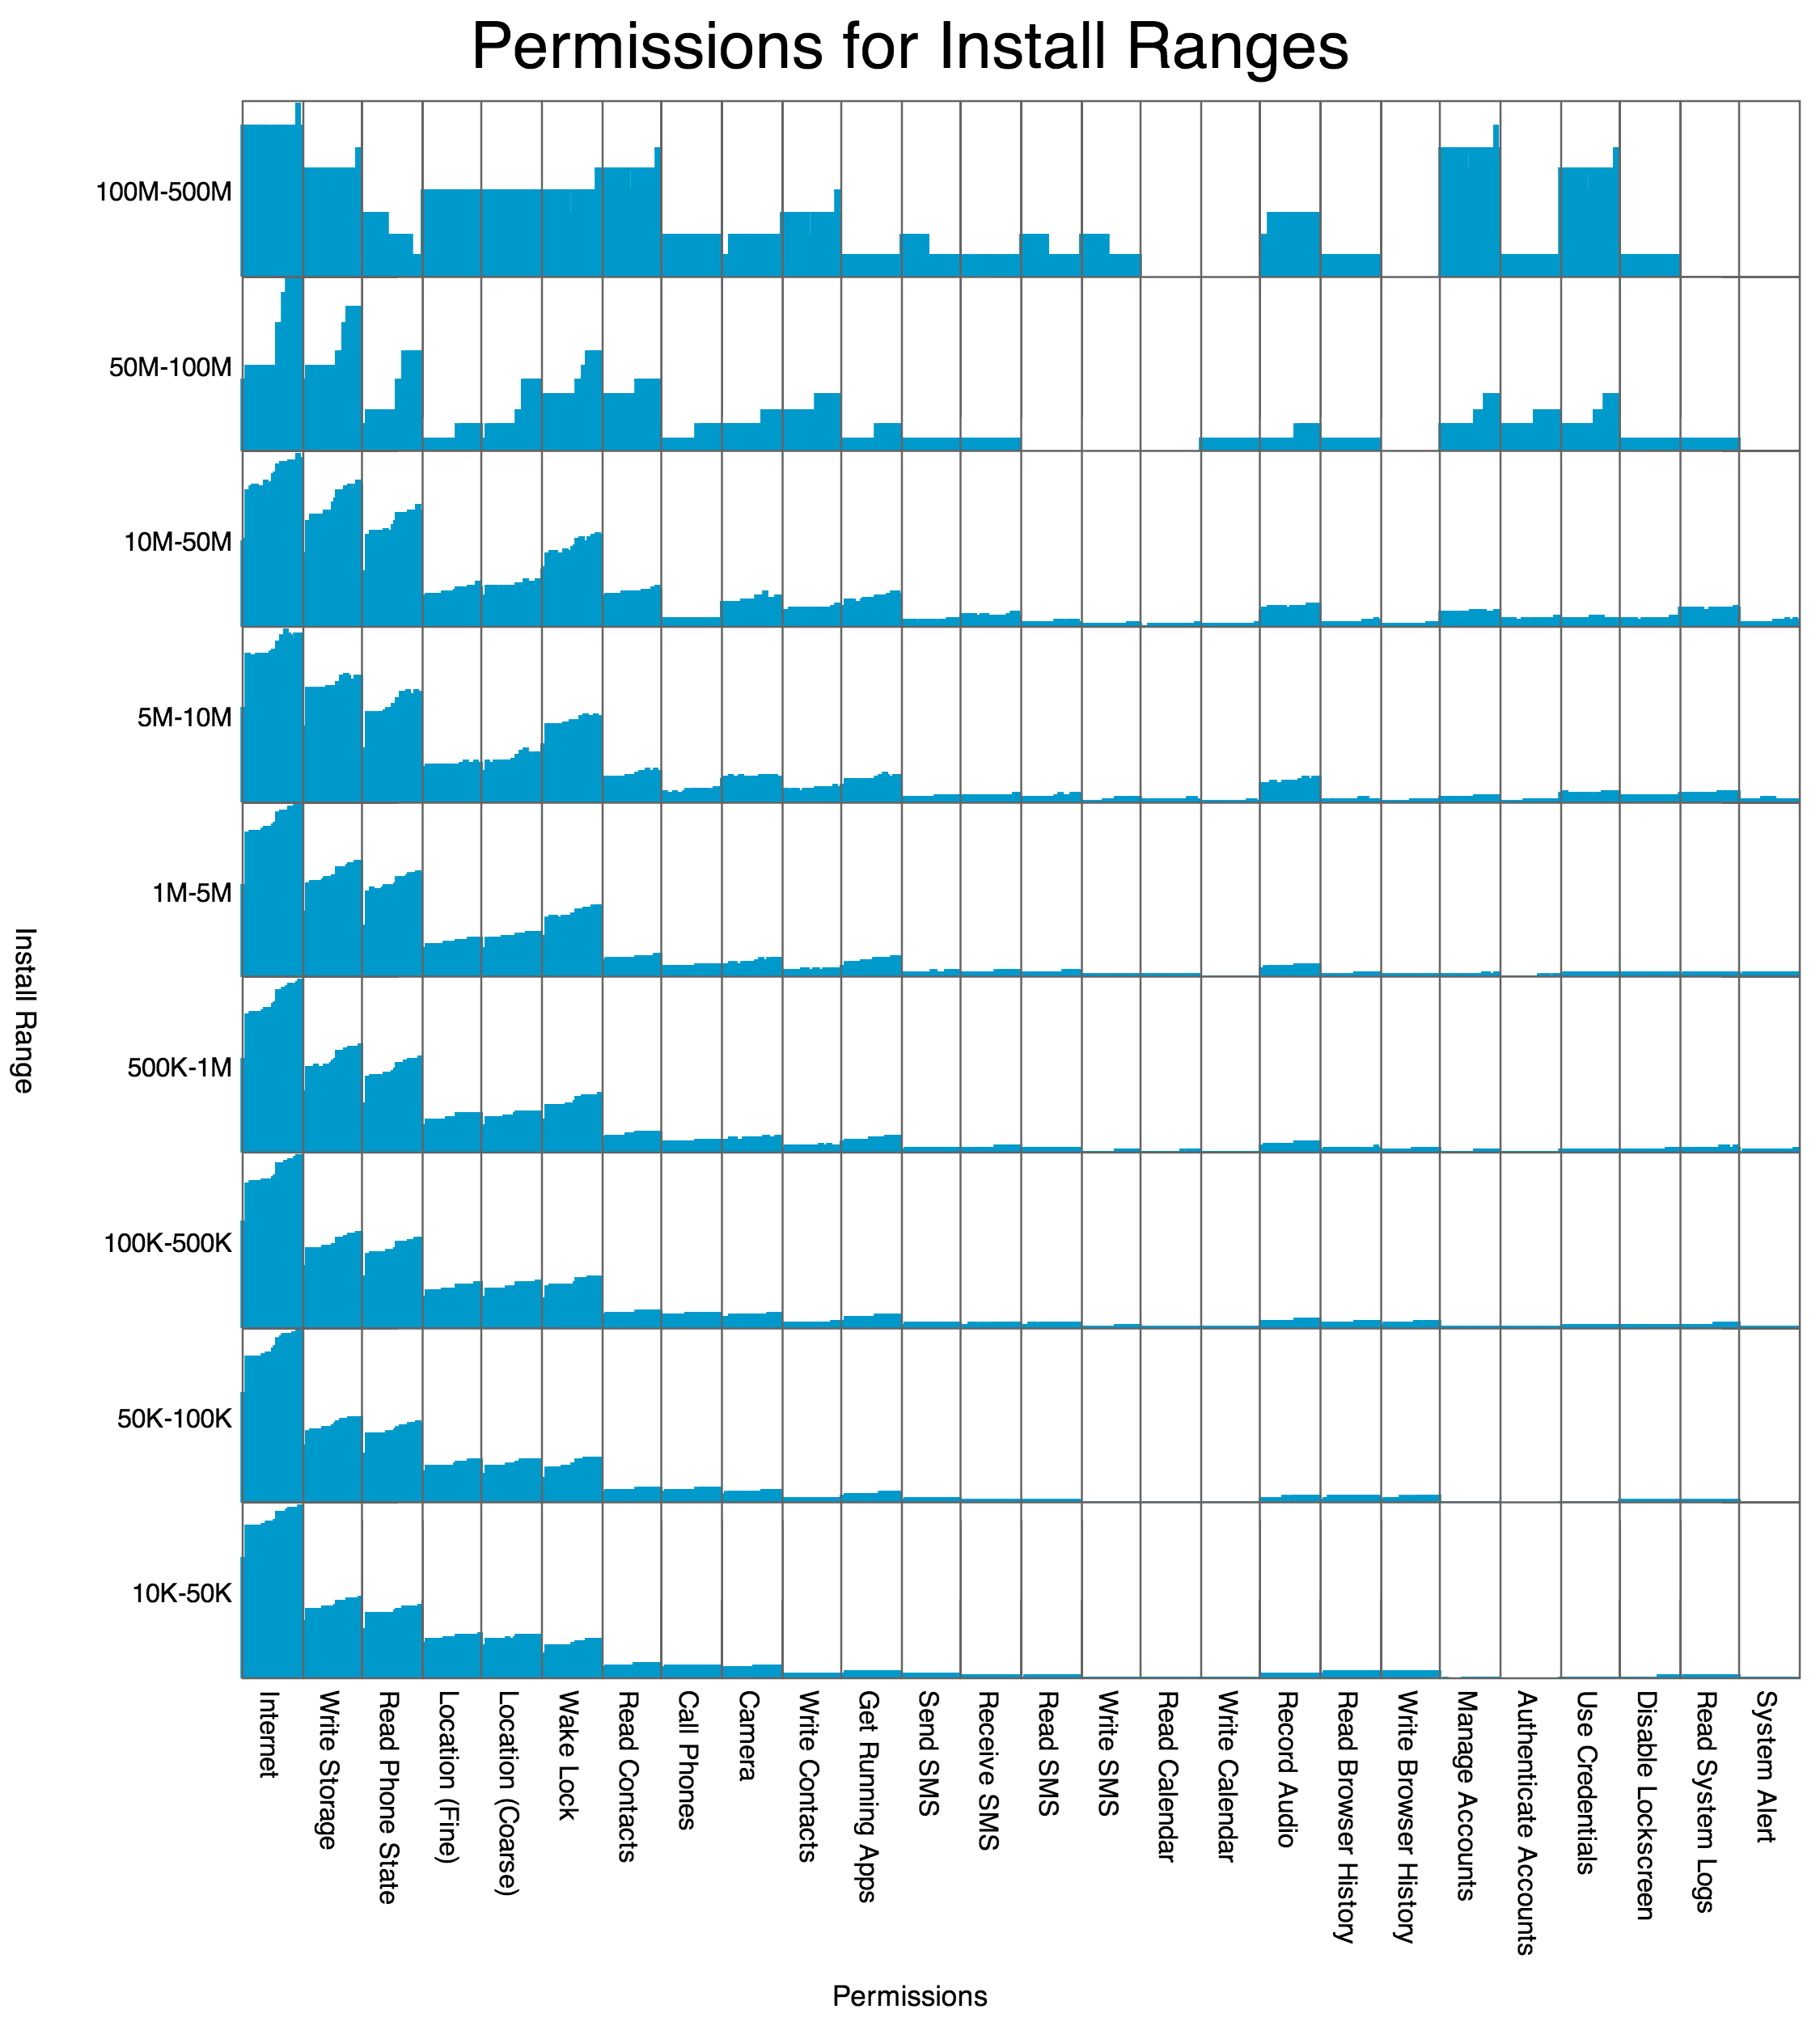
\includegraphics[width=1.0\columnwidth]{figs/PermissionsforInstallRanges}
\caption{Permission Fingerprints of apps with different ranges of install counts}
\label{fig:topappsfingerprint}
\end{center}
\end{figure}



\section{Conclusion}
We have demonstrated several key points in this analysis. First, we demonstrated that Permission Fingerprints often correlate with their expected behavior, but found key instances where these did not, especially with respect to PII. We then demonstrated that different classes of malware have permission fingerprints that correlate strongly with their expected behavior, but vary heavily from the rest of the GPStore. However, we noted that \textit{SMS} malware only needed one key permission to operate - one that was ultimately not terribly uncommon in many categories, and Info Theft apps had a permission fingerprint that does not ultimately stick out in the GPStore as a whole. When analyzing the top apps, we found many opportunities for Info Theft malware to imitate their permission fingerprints.

%We have established the limits of Permission Fingerprints: Whereas they list capabilities, they are broad, and do not offer the insight necessary to identify malicious behavior. We have demonstrated that malicious behavior and acceptable behavior can come from the same Permissions. This is ultimately due to two main issues, Permissions do not address the context of use, nor what is done with the data after granting it. These two ideas, context and use, are some defining aspects of the User-App Agreement.
\chapter{Framework Evaluation}
\label{sec:framework}

With AndroMEDA, we attempt to build on top of the Android Permission system, to do a better job at enforcing the User-App Agreement. The main reasons why the Permission System failed to differentiate between malware and normal software can be seen as a lack of context and understanding of use. When an app requests a permission, it is granted to the app reguardless of any context - at any time, and reguardless of user consent. The data, after being requested, ultimately can be manipulated and trasmitted to any party without user consent. 

Projects like TaintDroid\citep{enck2010taintdroid} have begun to address the flow of personal data, which aids in the user understanding the use of data. Ultimately, however, much more can be done to address both context and use, which AndroMEDA attempts to address. By instrumenting API calls, AndroMEDA can both inspect context and to some extent use of personal data and other system actions, and by visualizing this information to the user, provides them with the ability to evaulate whether the User-App Agreement has been broken.

\section{Test Introduction}
To test the effectiveness of AndroMEDA at detecting malicious behavior, we begin with testing apps from the Android Malware Genome Project\citep{zhou2012dissecting}. Unfortunately, we found only 31 of the nearly 1300 samples were designed for Android 2.3 and above, and not a single one targeted Android 4.0 or above. Furthermore, we found many of the samples simply did not run anymore, due to deprecated APIs and other poor coding techniques. 

To test a future-malware oriented framework, it would be ideal to have more sophisticated malware. Rootkits and Premium SMS malware have been addressed by recent versions of Android, so we focus on what we believe to be the future of malware on Android: Sophisticated Info Stealing Apps. We introduce a novel sample of info stealing malware, embedded inside of existing software - designed to silently steal PII and upload it to a remote location. We build off of concepts like SoundComber\citep{schlegel2011soundcomber}
\chapter{Conclusion and Future Work}
\label{sec:conclusion}
\section{Conclusion}
AndroMEDA helps users understand the context in which their Personally Identifiable Information is used, which allows them to make more informed decisions on whether an app is action maliciously or not. 

In this paper, we introduced 3 key items:
\subsection{User-App Agreement}
%We analyze the state of Android and Permissions, and conclude the need to address the User-App Agreement, which is a framework for consenting and trusting specific actions an app may take. It lies at the heart of classifying Info Theft Malware. Android Permissions address the capabilities of an app, but fail to address the context and use of those capabilities, which are cruicial to trusting an app's actions.

We analyzed the current Android security framework: The Permission System, and found it's main flaws were it's lack of addressing context and use, which we generalize into the User-App Agreement - a framework for consenting and trusting specific actions an app may take. Whereas Android Permissions exceeded at defining general capabilities of an app, and these capabilities go a long way in shaping the User-App Agreement, they fail at addressing the context in which the permissions are used, and what they are used for.

\subsection{\temp{AndroidMarketDB}}
To perform a full analysis of the current state of Android Permissions, we use a novel dataset, \temp{AndroidMarketDB}. By analyzing more than 80\% of apps in the Google Play Store, we are able to better understand the interrelationship of permissions and expected behavior. We produce key insights as to the popularity of apps vs their PII permissions, and when apps deviate from their expected behavior - potentially violating the User-App Agreement. We then analyze a comprehensive malware dataset using the same techniques, and find that many types of malware can be identified purely by it's permission fingerprint. We conclusively show the connection between Permissions and Expected Behavior are present, but not strong enough to differentiate between Info Theft Malware and many popular apps.

\subsection{AndroMEDA}
Building off the concept of the User-App Agreement, we introduce AndroMEDA. Key parts of the User-App Agreement were previously unnoticable to the user until AndroMEDA. By giving the user more information on the context and use of permissions, they can evaluate whether they trust those actions, and ultimately whether the app is acting maliciously or not. This, in turn, helps mitigate Info Theft Malware on Android.

\section{Future Work}
\label{sec:futurework}
AndroMEDA is, ultimately, not a silver bullet at detecting all Android malware. Projects like TaintDroid and TISSA provide functionality that would greatly enhance the abilities of AndroMEDA to visualize context and use of permissions to the user, and allow them to take action against it. 

AndroMEDA could also benefit greatly from the probablistic modeling of pBMDs and Crowdroid, in correlating user action with permission behavior. These would not replace the need to alert the user, but rather be able to better dictate when to put different classes of alerts to the user, as ultimately the decision of what is malware is up to them.

The weath of data in \temp{AndroidMarketDB} was also not fully explored. We are currently interested in seeing if specific keywords in user reviews correlate with malicious software, or other problematic apps. Many more areas of metadata, like the description, developer, etc, can be further explored, to see if it gives additional insight into the nature of malware on Android.

\appendix*

\chapter{}
\section{Android Permissions}

\begin{small}
\begin{longtable}{p{3cm}|p{8cm}|p{2.5cm}|p{1.5cm}}
%\begin{tabular}{p{2cm}|p{3cm}|p{1cm}|p{8.5cm}}
Name & ID & Severity &3rd Party Usable \\
\hline

Bind Wallpaper & \textit{android.permission.\-BIND\_WALLPAPER} & signatureOrSystem & no \\
View Google Services & \textit{com.google.android.providers.gsf.permission.\-READ\_GSERVICES} & none & yes \\
Force Back & \textit{android.permission.\-FORCE\_BACK} & signatureOrSystem & no \\
Read Calendar & \textit{android.permission.\-READ\_CALENDAR} & dangerous & yes \\
Read Frame Buffer & \textit{android.permission.\-READ\_FRAME\_BUFFER} & signature & no \\
NFC & \textit{android.permission.\-NFC} & dangerous & yes \\
Read Sync Stats & \textit{android.permission.\-READ\_SYNC\_STATS} & none & yes \\
Battery Stats & \textit{?android.permission.\-BATTERY\_STATS} & none & yes \\
Internet & \textit{android.permission.\-INTERNET} & dangerous & yes \\
Change Config & \textit{android.permission.\-CHANGE\_CONFIGURATION} & dangerous & yes \\
Google Auth - Docs & \textit{com.google.android.googleapps.permission.\-GOOGLE\_AUTH.writely} & dangerous & yes \\
Test & \textit{android.permission.\-HARDWARE\_TEST} & signature & no \\
Read Google Contacts & \textit{com.google.android.googleapps.permission.\-GOOGLE\_AUTH.cp} & dangerous & yes \\
Read GTalk & \textit{com.google.android.providers.talk.permission.\-READ\_ONLY} & dangerous & yes \\
Google Auth - Calendar & \textit{com.google.android.googleapps.permission.\-GOOGLE\_AUTH.cl} & dangerous & yes \\
Bind Input & \textit{android.permission.\-BIND\_INPUT\_METHOD} & signature & no \\
Set Time Zone & \textit{android.permission.\-SET\_TIME\_ZONE} & dangerous & yes \\
Access Cache & \textit{android.permission.\-ACCESS\_CACHE\_FILESYSTEM} & signatureOrSystem & no \\
Write Sync Settings & \textit{android.permission.\-WRITE\_SYNC\_SETTINGS} & dangerous & yes \\
Change Data Settings & \textit{android.permission.\-CHANGE\_BACKGROUND\_DATA\_SETTING} & signature & no \\
Write Google Services & \textit{android.permission.\-WRITE\_GSERVICES} & signatureOrSystem & no \\
Inject Events & \textit{android.permission.\-INJECT\_EVENTS} & signature & no \\
Bind Device Admin & \textit{android.permission.\-BIND\_DEVICE\_ADMIN} & signature & no \\
Force Stop & \textit{android.permission.\-FORCE\_STOP\_PACKAGES} & signature & no \\
Write GTalk & \textit{com.google.android.providers.talk.permission.\-WRITE\_ONLY} & dangerous & yes \\
Write Secure Settings & \textit{android.permission.\-WRITE\_SECURE\_SETTINGS} & signatureOrSystem & no \\
Call All Numbers & \textit{android.permission.\-CALL\_PRIVILEGED} & signatureOrSystem & no \\
Broadcast App Removed & \textit{android.permission.\-BROADCAST\_PACKAGE\_REMOVED} & signatureOrSystem & no \\
System Alert & \textit{android.permission.\-SYSTEM\_ALERT\_WINDOW} & dangerous & yes \\
Location - Extra & \textit{android.permission.\-ACCESS\_LOCATION\_EXTRA\_COMMANDS} & none & yes \\
Brick & \textit{android.permission.\-BRICK} & signature & no \\
Dump System & \textit{android.permission.\-DUMP} & signatureOrSystem & no \\
Shutdown & \textit{android.permission.\-SHUTDOWN} & signature & no \\
Change WiFi & \textit{android.permission.\-CHANGE\_WIFI\_STATE} & dangerous & yes \\
Receive SMS & \textit{android.permission.\-RECEIVE\_SMS} & dangerous & yes \\
Modify Phone & \textit{android.permission.\-MODIFY\_PHONE\_STATE} & signatureOrSystem & no \\
Read Attachment & \textit{com.google.android.gm.permission.\-READ\_ATTACHMENT\_PREVIEW} & signature & no \\
Manage Accounts & \textit{android.permission.\-ACCOUNT\_MANAGER} & signature & no \\
Read GMail & \textit{com.google.android.gm.permission.\-READ\_GMAIL} & signature & no \\
Animation Scale & \textit{android.permission.\-SET\_ANIMATION\_SCALE} & dangerous & yes \\
Set Process Limit & \textit{android.permission.\-SET\_PROCESS\_LIMIT} & dangerous & yes \\
Move Package & \textit{android.permission.\-MOVE\_PACKAGE} & signatureOrSystem & no \\
Google Auth - Other & \textit{com.google.android.googleapps.permission.\-GOOGLE\_AUTH.OTHER\_SERVICES} & dangerous & yes \\
Debug App & \textit{android.permission.\-SET\_DEBUG\_APP} & ? & no \\
Install DRM & \textit{android.permission.\-INSTALL\_DRM} & none & yes \\
Bluetooth & \textit{android.permission.\-BLUETOOTH} & dangerous & yes \\
Camera & \textit{android.permission.\-CAMERA} & dangerous & yes \\
Set Wallpaper Hints & \textit{android.permission.\-SET\_WALLPAPER\_HINTS} & none & yes \\
Reboot & \textit{android.permission.\-REBOOT} & signatureOrSystem & no \\
Broadcast WAP & \textit{android.permission.\-BROADCAST\_WAP\_PUSH} & signature & no \\
Google Auth - Maps & \textit{com.google.android.googleapps.permission.\-GOOGLE\_AUTH.local} & dangerous & yes \\
View Network & \textit{android.permission.\-ACCESS\_NETWORK\_STATE} & none & yes \\
Status Bar & \textit{android.permission.\-STATUS\_BAR} & signatureOrSystem & no \\
Write User Dictionary & \textit{android.permission.\-WRITE\_USER\_DICTIONARY} & none & yes \\
Read Browser History & \textit{com.android.browser.permission.\-READ\_HISTORY\_BOOKMARKS} & dangerous & yes \\
Access DRM & \textit{android.permission.\-ACCESS\_DRM} & signature & no \\
Record Audio & \textit{android.permission.\-RECORD\_AUDIO} & dangerous & yes \\
Write Contacts & \textit{android.permission.\-WRITE\_CONTACTS} & dangerous & yes \\
Send Gmail & \textit{com.google.android.gm.permission.\-AUTO\_SEND} & signature & no \\
Control Location & \textit{android.permission.\-CONTROL\_LOCATION\_UPDATES} & signatureOrSystem & no \\
Bind Widgets & \textit{android.permission.\-BIND\_APPWIDGET} & signatureOrSystem & no \\
Send Linux Signals & \textit{android.permission.\-SIGNAL\_PERSISTENT\_PROCESSES} & dangerous & yes \\
Install Location Provider & \textit{android.permission.\-INSTALL\_LOCATION\_PROVIDER} & signatureOrSystem & no \\
Google Auth - Drive & \textit{com.google.android.googleapps.permission.\-GOOGLE\_AUTH.wise} & dangerous & yes \\
Start On Boot & \textit{android.permission.\- RECEIVE\_BOOT\_COMPLETED} & none & yes \\
Clear Phone & \textit{android.permission.\-MASTER\_CLEAR} & signatureOrSystem & no \\
Read Input State & \textit{android.permission.\-READ\_INPUT\_STATE} & signature & no \\
Internal System UI & \textit{android.permission.\-INTERNAL\_SYSTEM\_WINDOW} & signature & no \\
Manage App Token & \textit{android.permission.\-MANAGE\_APP\_TOKENS} & signature & no \\
Access Email & \textit{com.android.email.permission.\-ACCESS\_PROVIDER} & ? & no \\
Subscribe Feeds & \textit{android.permission.\-WRITE\_SETTINGS} & dangerous & yes \\
SIP & \textit{android.permission.\-USE\_SIP} & dangerous & yes \\
Google Auth - AppEngine & \textit{com.google.android.googleapps.permission.\-GOOGLE\_AUTH.ah} & dangerous & yes \\
Write APM & \textit{android.permission.\-WRITE\_APN\_SETTINGS} & dangerous & yes \\
Access Surface & \textit{android.permission.\-ACCESS\_SURFACE\_FLINGER} & signature & no \\
Factory Test & \textit{android.permission.\-FACTORY\_TEST} & signature & no \\
Google Auth - Gmail & \textit{com.google.android.googleapps.permission.\-GOOGLE\_AUTH.mail} & dangerous & yes \\
Read System Logs & \textit{android.permission.\-READ\_LOGS} & dangerous & yes \\
Process Outgoing Calls & \textit{android.permission.\-PROCESS\_OUTGOING\_CALLS} & dangerous & yes \\
Update Device Stats & \textit{android.permission.\-UPDATE\_DEVICE\_STATS} & signature & no \\
Write Calendar & \textit{android.permission.\-WRITE\_CALENDAR} & dangerous & yes \\
Google Auth - Youtube & \textit{com.google.android.googleapps.permission.\-GOOGLE\_AUTH.youtube} & dangerous & yes \\
Read Feeds & \textit{android.permission.\-SUBSCRIBED\_FEEDS\_READ} & none & yes \\
Manage Accounts & \textit{android.permission.\-MANAGE\_ACCOUNTS} & dangerous & yes \\
Send SMS & \textit{android.permission.\-SEND\_SMS} & dangerous & yes \\
Google Auth - Blogger & \textit{com.google.android.googleapps.permission.\-GOOGLE\_AUTH.blogger} & dangerous & yes \\
Mock Location & \textit{android.permission.\-ACCESS\_MOCK\_LOCATION} & dangerous & yes \\
Change WiFi Multicast & \textit{android.permission.\-CHANGE\_WIFI\_MULTICAST\_STATE} & dangerous & yes \\
Access Passwords & \textit{com.google.android.googleapps.permission.\-ACCESS\_GOOGLE\_PASSWORD} & signatureOrSystem & no \\
Google Auth - All & \textit{com.google.android.googleapps.permission.\-GOOGLE\_AUTH.ALL\_SERVICES} & dangerous & yes \\
Write SMS & \textit{android.permission.\-WRITE\_SMS} & dangerous & yes \\
Get Running Apps & \textit{android.permission.\-GET\_TASKS} & dangerous & yes \\
Delete Packages & \textit{android.permission.\-DELETE\_PACKAGES} & signatureOrSystem
 & no \\
Access Checkins & \textit{android.permission.\-ACCESS\_CHECKIN\_PROPERTIES} & signatureOrSystem & no \\
Set Preferred Apps & \textit{android.permission.\-SET\_PREFERRED\_APPLICATIONS} & signature & no \\
Set Time & \textit{android.permission.\-SET\_TIME} & signatureOrSystem & no \\
Vibrate & \textit{android.permission.\-VIBRATE} & none & yes \\
Diagnostic & \textit{android.permission.\-DIAGNOSTIC} & signature & no \\
Call Phones & \textit{android.permission.\-CALL\_PHONE} & dangerous & yes \\
Flashlight & \textit{android.permission.\-FLASHLIGHT} & none & yes \\
Read Phone State & \textit{android.permission.\-READ\_PHONE\_STATE} & dangerous & yes \\
Location (Coarse) & \textit{android.permission.\-ACCESS\_COARSE\_LOCATION} & dangerous & yes \\
Clear App Data & \textit{android.permission.\-CLEAR\_APP\_USER\_DATA} & signature & no \\
Broadcast SMS & \textit{android.permission.\-BROADCAST\_SMS} & signatureOrSystem & no \\
Kill Background & \textit{android.permission.\-KILL\_BACKGROUND\_PROCESSES} & none & yes \\
Stop App Switching & \textit{android.permission.\-STOP\_APP\_SWITCHES} & signature & no \\
Access WiFi & \textit{android.permission.\-ACCESS\_WIFI\_STATE} & none & yes \\
Receive SMS & \textit{android.permission.\-RECEIVE\_MMS} & dangerous & yes \\
Wake Lock & \textit{android.permission.\-WAKE\_LOCK} & dangerous & yes \\
Write Browser History & \textit{com.android.browser.permission.\-WRITE\_HISTORY\_BOOKMARKS} & dangerous & yes \\
Delete Cache Files & \textit{android.permission.\-DELETE\_CACHE\_FILES} & signatureOrSystem & no \\
View Google Auth & \textit{com.google.android.googleapps.permission.\-GOOGLE\_AUTH} & none & yes \\
Read Accounts & \textit{android.permission.\-GET\_ACCOUNTS} & none & yes \\
Change Network & \textit{android.permission.\-CHANGE\_NETWORK\_STATE} & dangerous & yes \\
Read Sync Settings & \textit{android.permission.\-READ\_SYNC\_SETTINGS} & none & yes \\
Disable Lockscreen & \textit{android.permission.\-DISABLE\_KEYGUARD} & dangerous & yes \\
Write Gmail & \textit{com.google.android.gm.permission.\-WRITE\_GMAIL} & signature & no \\
Use Credentials & \textit{android.permission.\-USE\_CREDENTIALS} & dangerous & yes \\
Write Feeds & \textit{android.permission.\-SUBSCRIBED\_FEEDS\_WRITE} & dangerous & yes \\
Kill Background Apps & \textit{? android.permission.\-KILL\_BACKGROUND\_PROCESSES} & none & yes \\
Change Components & \textit{android.permission.\-CHANGE\_COMPONENT\_ENABLED\_STATE} & signature & no \\
Backup & \textit{android.permission.\-BACKUP} & signatureOrSystem & no \\
Google Auth - Finance & \textit{com.google.android.googleapps.permission.\-GOOGLE\_AUTH.finance} & dangerous & yes \\
Expand Status Bar & \textit{android.permission.\-EXPAND\_STATUS\_BAR} & none & yes \\
Bluetooth Admin & \textit{android.permission.\-BLUETOOTH\_ADMIN} & dangerous & yes \\
Location (Fine) & \textit{android.permission.\-ACCESS\_FINE\_LOCATION} & dangerous & yes \\
Youtube Username & \textit{com.google.android.googleapps.permission.\-GOOGLE\_AUTH.YouTubeUser} & dangerous & yes \\
Persist Activity (dep.) & \textit{android.permission.\-PERSISTENT\_ACTIVITY} & DEPRECATED & no \\
Reorder Tasks & \textit{android.permission.\-REORDER\_TASKS} & ? & no \\
Receive WAP Push & \textit{android.permission.\-RECEIVE\_WAP\_PUSH} & dangerous & yes \\
Receive C2DM & \textit{com.google.android.c2dm.permission.\-RECEIVE} & none & yes \\
Set Wallpaper & \textit{android.permission.\-SET\_WALLPAPER} & none & yes \\
Google Auth - Picasa & \textit{com.google.android.googleapps.permission.\-GOOGLE\_AUTH.lh2} & dangerous & yes \\
Read User Dictionary & \textit{android.permission.\-READ\_USER\_DICTIONARY} & dangerous & yes \\
Write Storage & \textit{android.permission.\-WRITE\_EXTERNAL\_STORAGE} & dangerous & yes \\
Get Package Size & \textit{android.permission.\-GET\_PACKAGE\_SIZE} & none & yes \\
Install Packages & \textit{android.permission.\-INSTALL\_PACKAGES} & signatureOrSystem & no \\
Authenticate Accounts & \textit{android.permission.\-AUTHENTICATE\_ACCOUNTS} & dangerous & yes \\
Set Alarm & \textit{com.android.alarm.permission.\-SET\_ALARM} & none & yes \\
Google Auth & \textit{com.google.android.googleapps.permission.\-GOOGLE\_AUTH.grandcentral} & dangerous & yes \\
Read Contacts & \textit{android.permission.\-READ\_CONTACTS} & dangerous & yes \\
CDMA Provisioning & \textit{android.permission.\-PERFORM\_CDMA\_PROVISIONING} & signatureOrSystem & no \\
Modify Audio & \textit{android.permission.\-MODIFY\_AUDIO\_SETTINGS} & dangerous & yes \\
Set Orientation & \textit{android.permission.\-SET\_ORIENTATION} & signature & no \\
Set Activity Watcher & \textit{android.permission.\-SET\_ACTIVITY\_WATCHER} & signature & no \\
Read SMS & \textit{android.permission.\-READ\_SMS} & dangerous & yes \\
Broadcast Sticky & \textit{android.permission.\-BROADCAST\_STICKY} & none & yes \\
Mount Filesystems & \textit{android.permission.\-MOUNT\_FORMAT\_FILESYSTEMS} & dangerous & yes \\
Clear App Cache & \textit{android.permission.\-CLEAR\_APP\_CACHE} & dangerous & yes \\
Mount Filesystems & \textit{android.permission.\-MOUNT\_UNMOUNT\_FILESYSTEMS} & dangerous & yes \\





%\end{tabular}
%\vspace{-0.2in}
\caption{All Android Permissions in the Google Play Store}
\label{tab:allperms}
%\vspace{-0.1in}
\end{longtable}
\end{small}



\backmatter

\bibliographystyle{abbrvnat}
%\bibliographystyle{latex8}
\bibliography{ref}

\end{document}
\endinput
%% End of file `thesis-ex.tex'.





%TODO:
% X  Add GPStore images
% X  Put GPSTORE reference in background
% X  put GPStore permission image in permissions
% X  put in footnote about Android 4.2 READ_STORAGE
% X  Expand on permission rejection in Permissions
% X  Find official source for improving rootkit protection, cite that later.
% X  Show some examples of SMS Trojan - FakeInst
% ?X Put in paragraph about our own malware dataset
% X  Make related works go Project, Shortcomings, Project SHortcomings, etc.
% X  Cite all security extensions in Architecture
%    Make goals of architecture a bullet list
% X  Include companion app in architecutre overview figure
% Talk more about market dataset.
% X  Include appendix of all permissions - just copypaste the spreadsheet, and reference it when we start talking about permissions
% X  Further talk about outliers in the GPStore thingie that personalization
%      https://play.google.com/store/apps/details?id=com.livewallpaper.livewallpaper.jjhearts
%      https://play.google.com/store/apps/details?id=com.fede.launcher
%      https://play.google.com/store/apps/details?id=wave.live.jwallpapers
% X  Reference the GPStore image in the marketanalysis when talking about popular apps
% X  Generate table of malware dataset and target SDKs, and use to talk about why it's useless.
% Use examples from UAA, turn them into malware, and demonstrate how easy it is to spot.
% conclusion: lack of malware dataset to test on. need to do usability studies.

% RESPONSES TO TODO
% Should we save the market pages above for future reference?




% ADD CONTRIBUTIONS To intro
% PUT IN conclusion how we proved contributions
% Merge 2.2 Malware and 2.2.1 Mobile Malware?
% Keep tense the same. PROOF READ. (especially chapter 3 intro)
% Cite numbers for 4.2 - monetery aservice attack
% Cite someone talking about the three main categories of malware
% Further discuss project shortcomings - It can't detect TapLogger.
% Just more statistics. maybe a table for chapter 4?
% Summary of related works into a table
% Do actual statistics? gah that'd be so hard. (Conclusion when we talk about malware fingerprints being easy to see)

% 
% 
%
% 
% 
% 
%
% 
% 
% 
%
% 
% 
% 
%
% 